\documentclass{article}

%------------------------------------------------------------------- PACKAGES -
\usepackage{amsmath,amsfonts,amssymb}
\usepackage{xspace}
\usepackage{graphicx}
\graphicspath{{./}{./figs/}}
\usepackage{natbib}
\bibpunct{(}{)}{;}{a}{}{,} % to follow the A&A style

\usepackage{hyperref}
% \hypersetup{
%   breaklinks=true,
%   colorlinks=true,
%   linkcolor=myLinkColor,
%   %anchorcolor=black,
%   citecolor=myLinkColor,
%   filecolor=myLinkColor,
%   menucolor=myLinkColor,
%   pagecolor=myLinkColor,
%   urlcolor=myLinkColor,
%   %backref=true,
%   %hyperindex=true
% }

\newcommand{\vocab}[1]{\textbf{#1}}

%---------------------------------------------------------------- TITLE PAGE -
%%% Requires opt_col_sm.jpg and titling package
\usepackage{titling} % \thetitle, \theauthor, \thedate for use in title page
%%% Custom commands to set title page content
\newcommand{\identifier}[1]{\def\theidentifier{#1}}
\newcommand{\revision}[1]{\def\therevision{#1}}

%%% Custom command to generate title page
\newcommand{\opttitlepage}{
\begin{titlepage}
\thispagestyle{plain}
\begin{center}
%
\vspace*{18mm}
{\bfseries\sffamily
  \Large\thetitle \\
  \vspace{6mm}
  \large\theidentifier \\ }
%
\vspace{17mm}
{\large\bfseries\sffamily \theauthor \\ }
%
\vspace{24mm}
{\large\bfseries\sffamily
  rev \therevision \\
  \vspace{6mm}
  \thedate \\ }
%
\vspace{36mm}

\includegraphics{opt_col_sm} \\
%
\end{center}
\end{titlepage}
}

%---------------------------------------------------------------- MATH MACROS -

% Notes:
%   \stackrel{top}{bot}
%   \overset{top}{base}
%   \underset{bot}{base}
%   \mathop{arg} - The argument is considered to be a single variable sized
%           math symbol for purposes of placing limits below (subscripts)
%           and above (superscripts) in display math style.

\makeatletter
\newcommand{\MathFuncName}[1]{{\operator@font #1}}
\newcommand{\MathFunc}[1]{\mathop{\operator@font #1}\nolimits}
\newcommand{\MathFuncWithLimits}[1]{\mathop{\operator@font #1}\limits}
\makeatother

\newcommand{\BF}[1]{\mathbf{#1}}         % math bold
%\newcommand{\RM}[1]{\mathrm{#1}}         % math roman
\newcommand{\SF}[1]{\mathsf{#1}}         % math sans-serif
\newcommand{\OP}[1]{{\MathFuncName{#1}}} % upright (*) for names
\newcommand{\Tag}[1]{\mathsf{#1}}        % math font for labels and tags
\newcommand{\BS}[1]{{\boldsymbol{#1}}}   % bold symbol (*)
\newcommand{\V}[1]{\boldsymbol{#1}}      % vector
\newcommand{\M}[1]{\mathbf{#1}}          % matrix
\newcommand{\T}{^\mathrm{T}}             % suffix for transpose
\newcommand{\I}{\mathrm{i}}              % roman 'i' for sqrt(-1)
\newcommand{\E}{\mathrm{e}}              % roman 'e' for exp(1)
\newcommand{\D}[1]{{\mathrm{d}#1}}       % integrand/differential
\newcommand{\ScaleAs}{\mathcal{O}}       % O(n)
\newcommand{\FT}[1]{\hat{#1}}            % Fourier transform
\newcommand{\TwoIPi}{2\,\I\,\pi}         % 2*i*pi
\renewcommand{\Re}{\MathFunc{Re}}        % real part
\renewcommand{\Im}{\MathFunc{Im}}        % imaginary part
\newcommand{\arc}{\MathFunc{arc}}        % length of arc
\newcommand{\rnd}{\MathFunc{rnd}}        % random
\newcommand{\sgn}{\MathFunc{sgn}}        % sign
\newcommand{\sinc}{\MathFunc{sinc}}      % cardinal sine
\newcommand{\Var}{\MathFunc{Var}}        % variance
\newcommand{\Cov}{\MathFunc{Cov}}        % covariance
\newcommand{\diag}{\MathFunc{diag}}      % diagonal
\newcommand{\tr}{\MathFunc{tr}}          % trace
% (*) enclosed in braces so that x_\BS{u} or x_\RM{name} works

\newcommand{\asterisk}{*}
\newcommand{\mathd}{\mathrm{d}}
\newcommand{\mathe}{\mathrm{e}}
\newcommand{\mathi}{\mathrm{i}}

\newcommand{\Paren}[1]{\left(#1\right)}
\newcommand{\Brack}[1]{\left[#1\right]}
\newcommand{\Brace}[1]{\left\{#1\right\}}

\newcommand{\PDer}[2]{\frac{\partial #1}{\partial #2}}
\newcommand{\QuadTerm}[2]{ #2\T\cdot #1\cdot #2}

\newcommand{\norm}[1]{\Vert #1\Vert}
\newcommand{\Norm}[1]{\left\Vert #1\right\Vert}
\newcommand{\bigNorm}[1]{\bigl\Vert #1\bigr\Vert}
\newcommand{\BigNorm}[1]{\Bigl\Vert #1\Bigr\Vert}

\newcommand{\abs}[1]{\vert #1\vert}
\newcommand{\Abs}[1]{\left\vert #1\right\vert}
\newcommand{\bigAbs}[1]{\bigl\vert #1\bigr\vert}
\newcommand{\BigAbs}[1]{\Bigl\vert #1\Bigr\vert}

\newcommand{\avg}[1]{\langle #1\rangle}
\newcommand{\Avg}[1]{\left\langle #1\right\rangle}
\newcommand{\bigAvg}[1]{\bigl\langle #1\bigr\rangle}
\newcommand{\BigAvg}[1]{\Bigl\langle #1\Bigr\rangle}
\newcommand{\expected}[1]{\mathrm{E}\{#1\}}
\newcommand{\Expected}[1]{\mathrm{E}\left\{#1\right\}}
\newcommand{\bigExpected}[1]{\mathrm{E}\bigl\{#1\bigr\}}
\newcommand{\BigExpected}[1]{\mathrm{E}\Bigl\{#1\Bigr\}}

\newcommand{\complex}[1]{\underline{#1}}

\newcommand{\argmin}{\MathFuncWithLimits{arg\,min}}
\newcommand{\argmax}{\MathFuncWithLimits{arg\,max}}

% Sets:
\newcommand{\Reals}{\mathbb{R}}
\newcommand{\Integers}{\mathbb{Z}}
\newcommand{\Complexes}{\mathbb{C}}
\newcommand{\Rationals}{\mathbb{Q}}

%\newcommand\bydef{\equiv}
%\newcommand\bydef{\triangleq}
\newcommand{\bydef}{\stackrel{\mathrm{def}}{=}}

% Common abbreviation:
\newcommand{\cf}{\textit{c.f.}\xspace}
\newcommand{\ie}{\textit{i.e.}\xspace}
\newcommand{\etc}{etc.\xspace}
\newcommand{\apriori}{\textit{a priori}\xspace}
\newcommand{\wrt}{with respect to\xspace}
\newcommand{\Eq}[1]{Eq.~(\ref{#1})}
\newcommand{\Fig}[1]{Fig.~\ref{#1}}
\newcommand{\Tab}[1]{Tab.~\ref{#1}}

%------------------------------------------------------------------------------
% Ref: Alexander R. Perlis., "A complement to \smash, \llap, and \rlap,"
%      TUGboat, Vol. 22, pp. 350-352, 2001.
%      <http://math.arizona.edu/~aprl/publications/mathclap/>
%
% For comparison, the existing overlap macros:
% \def\llap#1{\hbox to 0pt{\hss#1}}
% \def\rlap#1{\hbox to 0pt{#1\hss}}
  \def\clap#1{\hbox to 0pt{\hss#1\hss}}
  \def\mathllap{\mathpalette\mathllapinternal}
  \def\mathrlap{\mathpalette\mathrlapinternal}
  \def\mathclap{\mathpalette\mathclapinternal}
  \def\mathllapinternal#1#2{\llap{$\mathsurround=0pt#1{#2}$}}
  \def\mathrlapinternal#1#2{\rlap{$\mathsurround=0pt#1{#2}$}}
  \def\mathclapinternal#1#2{\clap{$\mathsurround=0pt#1{#2}$}}

%------------------------------------------------------------------------------
%
% The commands:
%
%   \Symbol{\COMMAND}{SYMBOL}
%   \SymbolWithLabel{\COMMAND}{SYMBOL}{LABEL}
%   \VectorSymbol{\COMMAND}{SYMBOL}
%   \VectorSymbolWithLabel{\COMMAND}{SYMBOL}{LABEL}
%   \MatrixSymbol{\COMMAND}{SYMBOL}
%   \MatrixSymbolWithLabel{\COMMAND}{SYMBOL}{LABEL}
%
% defines a macro \COMMAND which can be used with an optional argument
% with the indexes.  For instance:
%
%   \Symbol{\QE}{\eta}
%   \QE      is just \eta
%   \QE[idx] is an \eta with a subscript 'idx'
%
%   \SymbolWithLabel{\Eint}{E}{int}
%   \Eint      is just an E with a subscript 'int'
%   \Eint[idx] is an E with a superscript 'int' and subscript 'idx'
%
% Note that SYMBOL and LABEL can be macros which get expanded.
% The \Symbol and \SymbolWithLabel can be globally modified to change the
% notation and/or the way their optional argument appears (as subscript, or
% as a list of arguments to mimic syntax of a given programming language).
%
\makeatletter

\newcommand{\@SymbolBuilderWithLabel}[4]{%
  %% Define \my@tempa to be arg #1 without backslash:
  \begingroup \escapechar\m@ne\xdef\my@tempa{\string#1}\endgroup
  %\typeout{TempA: '\my@tempa'}
  %% Make sure macro is not yet defined:
  \expandafter\@ifundefined{\my@tempa}{%
    %% Define 'public' command \COMMAND:
    \def\my@tempb{[} % to avoid mismatching below
    \expandafter\edef\csname\my@tempa\endcsname{%
      \noexpand\@ifnextchar\my@tempb%
          {\csname\my@tempa @b\endcsname}%
          {\csname\my@tempa @a\endcsname}%
    }
    %% Define 2 'private' commands \COMMAND@a and \COMMAND@b[#1] to work
    %% with the 'public' one:
    \expandafter\def\csname\my@tempa @a\endcsname{%
      {#2}_{#4}%
    }
    \expandafter\def\csname\my@tempa @b\endcsname[##1]{%
      {{#3}^{#4}_{##1}}%
    }
  }{\@latex@error{\noexpand#1is already defined}\@ehc}%
}
\newcommand{\@SymbolBuilder}[3]{% see \@SymbolBuilderWithLabel for comments
  \begingroup \escapechar\m@ne\xdef\my@tempa{\string#1}\endgroup
  \expandafter\@ifundefined{\my@tempa}{%
    \def\my@tempb{[}
    \expandafter\edef\csname\my@tempa\endcsname{%
      \noexpand\@ifnextchar\my@tempb%
          {\csname\my@tempa @b\endcsname}%
          {\csname\my@tempa @a\endcsname}%
    }
    \expandafter\def\csname\my@tempa @a\endcsname{%
      #2%
    }
    \expandafter\def\csname\my@tempa @b\endcsname[##1]{%
      {{#3}_{##1}}%
    }
  }{\@latex@error{\noexpand#1is already defined}\@ehc}%
}

\newcommand{\SymbolWithLabel}[3]{%
  \@SymbolBuilderWithLabel{#1}{#2}{#2}{#3}}
\newcommand{\Symbol}[2]{%
  \@SymbolBuilder{#1}{#2}{#2}}

\newcommand{\VectorSymbolWithLabel}[3]{%
  \@SymbolBuilderWithLabel{#1}{\V{#2}}{#2}{#3}}
\newcommand{\VectorSymbol}[2]{%
  \@SymbolBuilder{#1}{\V{#2}}{#2}}

\newcommand{\MatrixSymbolWithLabel}[3]{%
  \@SymbolBuilderWithLabel{#1}{\M{#2}}{#2}{#3}}
\newcommand{\MatrixSymbol}[2]{%
  \@SymbolBuilder{#1}{\M{#2}}{#2}}

\makeatother

%------------------------------------------------------------------- NOTATIONS -

\newcommand{\ComplexVis}{V}
\newcommand{\VisPhase}{\varphi}
%\newcommand{\VisAmplitude}{?}
\newcommand{\Powerspectrum}{S}
\newcommand{\Bispectrum}{B}
\newcommand{\PhaseClosure}{\beta}
\newcommand{\Freq}{\nu}               % spatial frequency
\newcommand{\VFreq}{\V{\Freq}}
\newcommand{\Dirn}{\theta}            % view direction
\newcommand{\VDirn}{\V{\Dirn}}
\newcommand{\Posn}{r}                 % projected position
\newcommand{\VPosn}{\V{\Posn}}
\newcommand{\Time}{t}                 % instantaneous time

\newcommand{\uv}{$(u,v)$\xspace}

\newcommand{\Image}{I}
\newcommand{\Param}{x}
\newcommand{\VParam}{\V{\Param}}
\newcommand{\Gain}{g}
\newcommand{\VGain}{\V{\Gain}}
\newcommand{\GainAmplitude}{\tau}
\newcommand{\GainPhase}{\phi}
\newcommand{\GainSquaredModulus}{\rho}
\newcommand{\OPD}{\delta}
\newcommand{\OPDmean}{\bar{\delta}}
\newcommand{\OPDstdev}{{\sigma_{\delta}}}
\newcommand{\BasisFunc}{b}
%\newcommand{\PixelGrid}{\mathcal{G}}
\newcommand{\FreqSet}{\mathcal{L}}  % set of observed spatial frequencies
\newcommand{\BaseSet}{\mathcal{B}}  % set of telescope pairs that contribute
                                    % to a particular baseline
\newcommand{\ApertureList}{\mathcal{A}} % list of aperture indexes
\newcommand{\ExposureList}{\mathcal{E}} % list of exposures
\newcommand{\Baseline}{B}
\newcommand{\MaxBaseline}{\Baseline_\Tag{max}}
\newcommand{\SuperResolutionFactor}{\xi}
\newcommand{\FeasibleSet}{\mathcal{X}}

% Grid for model parameters:
%\newcommand{\Grid}[1]{\breve{#1}}
\newcommand{\Grid}[1]{\stackrel{%
    {\fboxsep0.09em{\vbox{\hbox{\fbox{}}\vskip0pt}}}}{#1}}

\newcommand{\OTF}{G} % Optical Transfer Function


% Wavelength:
\Symbol{\Wavelength}{\lambda}
\Symbol{\GridWavelength}{\Grid{\Wavelength}}

% 2-D angular position / view direction:
\newcommand{\DirLetter}{a}
\Symbol{\Dir}{\V{\DirLetter}}
\Symbol{\GridDir}{\Grid{\V{\DirLetter}}}

% Global vector of parameters:
\newcommand{\ParamLetter}{x}
\VectorSymbol{\X}{\ParamLetter}

\MatrixSymbol{\XForm}{T}
\MatrixSymbol{\OTFop}{\OTF}
\MatrixSymbol{\DFTop}{F}
\MatrixSymbol{\InterpOp}{R}
\MatrixSymbol{\ModelOp}{A}
\MatrixSymbol{\PSFop}{H}
\MatrixSymbol{\ApodizationOp}{S}

% Point spread function:
\Symbol{\PSF}{h}
\VectorSymbolWithLabel{\Xpsf}{x}{\Tag{psf}}

% Data:
\newcommand{\DataLetter}{y}
\VectorSymbol{\Data}{\DataLetter}

% Model:
\VectorSymbol{\Model}{m}

% Errors:
\VectorSymbol{\Error}{e}

% Residuals:
\VectorSymbol{\Residual}{r}

% Tags:
\newcommand{\DataTag}{\Tag{data}}
\newcommand{\PriorTag}{\Tag{prior}}
\newcommand{\ErrorTag}{\Tag{err}}
\newcommand{\ModelTag}{\Tag{model}}
\newcommand{\MlTag}{\Tag{ML}}
\newcommand{\MapTag}{\Tag{MAP}}
\newcommand{\PowerspectrumTag}{\Tag{ps}}
\newcommand{\BispectrumTag}{\Tag{bisp}}
\newcommand{\PhaseClosureTag}{\Tag{cl}}
\newcommand{\BestTag}{+}

% Constraints:
\newcommand{\DataLevel}{\eta_\DataTag}
\newcommand{\PriorLevel}{\eta_\PriorTag}

% Covariances and weighting matrices:
\MatrixSymbolWithLabel{\Cerror}{C}{\ErrorTag}
\MatrixSymbolWithLabel{\Werror}{W}{\ErrorTag}
\MatrixSymbolWithLabel{\Cprior}{C}{\PriorTag}
\MatrixSymbolWithLabel{\Wprior}{W}{\PriorTag}
\MatrixSymbol{\Identity}{I}

% Penalty function:
\newcommand{\Fcost}{f}
\newcommand{\Fml}{\Fcost_\MlTag}
\newcommand{\Fmap}{\Fcost_\MapTag}
\newcommand{\Fdata}{\Fcost_\DataTag}
\newcommand{\Fprior}{\Fcost_\PriorTag}
\newcommand{\Weight}{w}

% Field of View:
\newcommand{\FOV}{\Omega}

% Algorithm names:
%\newcommand{\Mira}{\textsc{Mira}\xspace}
\newcommand{\Mira}{MiRA\xspace}
\newcommand{\BSMEM}{BSMEM\xspace}
\newcommand{\Wisard}{\textsc{Wisard}\xspace}
\newcommand{\Macim}{\textsc{Macim}\xspace}
\newcommand{\Squeeze}{\textsc{Squeeze}\xspace}

\newcommand{\OIFITS}{OIFITS\xspace} % not OI-FITS

% Empty definitions for further redefinitions via \renewcommand:
\newcommand{\Tmp}{}
\newcommand{\TmpA}{}
\newcommand{\TmpB}{}
\newcommand{\TmpC}{}
\newcommand{\TmpD}{}
\newcommand{\TmpE}{}

%------------------------------------------------------------------------------

\begin{document}

\title{Unified Image Reconstruction Description}

\author{John Young and Eric Thi\'ebaut}

% \author{
% John Young \footnote{University of Cambridge, Cavendish Laboratory, JJ
%   Thomson Avenue, Cambridge CB3 0PA; jsy1001 (at) cam.ac.uk}\\
% Eric~Thi\'ebaut \footnote{Centre de Recherche Astrophysique de Lyon,
%   CNRS/UMR 5574, Observatoire de Lyon, Universit\'e Lyon 1, \'Ecole Normale
%   Sup\'{e}rieure de Lyon; thiebaut (at) obs.univ-lyon1.fr}}

\identifier{Opticon WP4 Deliverable 4.1}
\revision{0.1}
\date{\today}

\opttitlepage

\begin{abstract}
  This document provides background information to astronomers
  wishing to use image reconstruction algorithms specifically developed for
  optical (visible/IR) interferometry, such as \Mira, \Wisard, and \BSMEM. It
  should be read in conjunction with the algorithm-specific documentation and
  cookbooks that will also be provided as outputs of this Joint Research
  Activity. We describe image reconstruction from interferometric data with a
  focus on the specific problems encountered at optical wavelengths.  The
  challenging issues in image reconstruction from interferometric data are
  introduced in the context of a general inverse problem approach.  This
  framework is then used to describe the algorithms specifically developed for
  optical interferometry. Other topics of interest to users of these
  algorithms are also covered, including general descriptions of the inputs,
  outputs and user interactions needed for succesful image reconstruction.
\end{abstract}

\section{Introduction}

The technique of aperture synthesis imaging, when applied at optical (visible
and near-infrared) wavelengths, offers an invaluable capability to image
astrophysical processes on milliarcsecond angular scales. The state-of-the-art
optical interferometers capable of performing such observations, for example
VLTI~\citep{Glindemann_et_al-2000-VLTI} and
CHARA~\citep{tenBrummelaar_et_al-2005-CHARA}, are now mature instruments, and
have yielded a number of published images. However, the available image
reconstruction software tools are relatively difficult for inexperienced
astronomers to use, and this is a significant (but by no means the only)
factor limiting the number of model-independent images that are published.

This document has been produced as part of a Joint Research Activity (JRA),
funded by the EU Seventh Framework Programme, which aims to provide
user-friendly image reconstruction software, accessible to the entire
community, and compatible with the instrumental capabilities that will be
offered by VLTI and CHARA a few years hence. The main outputs of the JRA will
be modified versions of existing algorithms with a common user interface, test
input datasets representative of a range of interferometric instruments and
observation types, and cookbooks that guide new users through various example
image reconstruction tasks.

The purpose of this document is to provide relevant background information for
end-users of the image reconstruction software and cookbooks, and also for
researchers preparing the other JRA outputs. Specifically, we will introduce a
lexical and mathematical vocabulary for describing the algorithms, and provide
high-level descriptions of the algorithms with a focus on their inputs,
outputs, similarities and differences. To inform the design of the common user
interface, we also enumerate common failure modes and explain the nature of
any user interventions that may be required to ensure successful image
reconstruction.  A more detailed presentation of the mathematical background
is given by \citet{Thiebaut-2013-principles}.

Multi-telescope interferometers provide sparse measurements of the Fourier
transform of the brightness distribution of the observed objects (Section
\ref{sec:interferometric-data}). An inverse problem methodology (Section
\ref{sec:image-reconstruction}) can be used to reconstruct images from such
sparsely-sampled Fourier data.  At optical wavelengths, additional problems
arise due to incomplete Fourier phase information, and to the non-linearity of
the direct model of the data in terms of the image parameters.  These issues
have led to the development of specific algorithms based on similar inverse
problem approaches (Section \ref{sec:optical-interferometry}). The input
parameters required by these algorithms are summarised in
Section~\ref{sec:inputs}.

In the following sections, key terms are highlighted (here is an example of
the typography: \vocab{complex visibility}). Where several synonyms are in
common usage, the highlighted one is preferred for the JRA outputs.


%%%%%%%%%%%%%%%%%%%%%%%%%%%%%%%%%%%%%%%%%%%%%%%%%%%%%%%%%%%%%%%%%%%%%%%%%%%%%%%
%%%%%%%%%%%%%%%%%%%%%%%%%%%%%%%%%%%%%%%%%%%%%%%%%%%%%%%% INTERFEROMETRIC DATA %
%%%%%%%%%%%%%%%%%%%%%%%%%%%%%%%%%%%%%%%%%%%%%%%%%%%%%%%%%%%%%%%%%%%%%%%%%%%%%%%

\section{Interferometric Data}
\label{sec:interferometric-data}

The instantaneous output of an optical interferometer is the so-called
\vocab{complex visibility} $\ComplexVis_{j_1,j_2}(t)$ of the interference
fringes between the $j_1$-th and the $j_2$-th telescopes at instant
$t$~\citep{Monnier-2003-interferometry}:
\begin{equation}
  \label{eq:instantaneous-complex-visibility}
  \ComplexVis_{j_1,j_2}(t) = \Gain_{j_1}(t)^{\star} \, \Gain_{j_2}(t) \,
  \FT{\Image}\Paren{\VFreq_{j_1,j_2}(t)} \, .
\end{equation}
Here $\FT{\Image}(\VFreq)$ is the Fourier transform of $\Image(\VDirn)$, the
brightness distribution of the observed object in angular direction $\VDirn$,
and $\Gain_{j}(t)$ is the complex amplitude throughput for the light from the
$j$-th telescope. The spatial frequency $\VFreq_{j_1,j_2}(t) =
(\VPosn_{j_2}(t) - \VPosn_{j_1}(t))/\Wavelength$ is determined by the
projection of the baseline between the pair of telescopes $(j_1,j_2)$ onto the
plane perpendicular to the line of sight, and is inversely proportional to the
observing wavelength $\Wavelength$ (see Fig.~\ref{fig:layout}).

These equations assume that the diameters of the telescopes are much smaller
than their projected separation and that the object is an incoherent light
source.  An interferometer therefore provides sparse measurements of the
Fourier transform of the brightness distribution of the observed object.  The
top-left panel of \Fig{fig:dirty-map} shows an example of the sampling of
spatial frequencies by an interferometer.

In practice, the complex visibility is measured during a finite exposure
duration:
\begin{equation}
  \label{eq:measured-complex-visibility}
  \ComplexVis_{j_1,j_2,m}^\DataTag = \avg{\ComplexVis_{j_1,j_2}(t)}_{m}
  + \ComplexVis_{j_1,j_2,m}^\ErrorTag
\end{equation}
where $\avg{\,}_{m}$ denotes averaging during the $m$-th exposure and
$\ComplexVis_{j_1,j_2,m}^\ErrorTag$ stands for the errors due to noise and
modeling approximations.  The exposure duration is short enough to consider
the projected baseline $\VPosn_{j_2}(t) - \VPosn_{j_1}(t)$ as constant, thus:
\begin{equation}
  \label{eq:averaged-complex-visibility}
  \avg{\ComplexVis_{j_1,j_2}(t)}_{m} \simeq
  \OTF_{j_1,j_2,m}\,
  %\avg{\Gain_{j_1}(t)^{\star} \, \Gain_{j_2}(t)}_{m} \,
  \FT{\Image}\Paren{\VFreq_{j_1,j_2,m}}
\end{equation}
with $\VFreq_{j_1,j_2,m} = \avg{\VFreq_{j_1,j_2}(t)}_{m} \simeq
\VFreq_{j_1,j_2}(t_m)$, $t_m=\avg{t}_{m}$ the mean time of the observation and
$\OTF_{j_1,j_2,m} = \avg{\Gain_{j_1}(t)^{\star} \, \Gain_{j_2}(t)}_{m}$ the
effective \vocab{optical transfer function} (OTF). The fast variations of the
instantaneous OTF are mainly due to the random optical path differences (OPD)
caused by the atmospheric turbulence.

% In long baseline interferometry, two telescopes are separated by more than the
% outer scale of the turbulence, hence their OPDs are independent.  Furthermore,
% the exposure duration is much longer than the evolution time of the turbulence
% (a few $10\,$ms) and averaging can be approximated by expectation:
% \begin{displaymath}
%   %\OTF_{j_1,j_2,m} =
%   \avg{\Gain_{j_1}(t)^{\star} \, \Gain_{j_2}(t)}_{m}
%   \simeq \Expected{\Gain_{j_1}(t)^{\star}}_{m} \,
%   \Expected{\Gain_{j_2}(t)}_{m}
% \end{displaymath}
% with $\expected{}_{m}$ the expectation during the $m$-th exposure.  During
% this exposure, the phase of $\Gain_{j}(t)$ is
% $\GainPhase_{j}(t)=\GainPhase_{j,m} + (2\,\pi/\lambda)\,\OPD_j(t)$ with
% $\GainPhase_{j,m}=\avg{\GainPhase_{j}(t)}_{m}$ the static phase aberration and
% $\OPD_j(t)\sim\mathcal{N}(0,\sigma_{\OPD}^2)$ the OPD which is a zero-mean
% Gaussian variable with the same standard deviation for all telescopes
% \citep{Roddier1981}.  For a given telescope, the amplitude and phase of the
% complex throughput can be assumed independent, hence:
% \begin{displaymath}
%   \Expected{\Gain_{j}(t)}_{m}
%   \simeq  \Expected{\abs{\Gain_{j}(t)}}_{m} \, 
%   \bigExpected{\mathe^{\mathi\,\GainPhase_{j}(t)}}_{m}
%   \simeq \Gain_{j,m} \, \mathe^{-\frac{1}{2}\sigma_{\GainPhase}^2}
% \end{displaymath}
% with $\Gain_{j,m}=\abs{\Gain_{j}(t_m)}\,\exp(-\mathi\,\GainPhase_{j,m})$ and
% $\sigma_{\GainPhase}^2=(2\,\pi/\lambda)^2\,\sigma_{\OPD}^2$ the variance of
% the phase during an exposure.  The OTF is finally:
% \begin{equation}
%   \label{eq:mean-otf}
%   \OTF_{j_1,j_2,m} = \avg{\Gain_{j_1}(t)^{\star} \, \Gain_{j_2}(t)}_{m}
%   \simeq \Gain_{j_1,m}^{\star} \, \Gain_{j_2,m} \,
%   \mathe^{-\sigma_{\GainPhase}^2}\,.
% \end{equation}

% At long wavelengths (radio), the phase variation during each exposure is
% small, hence $\OTF_{j_1,j_2,m} \simeq \Gain_{j_1,m}^{\star} \,
% \Gain_{j_2,m}\not=0$.  If some means to calibrate the $\Gain_{j,m}$'s are
% available, then image reconstruction amounts to deconvolution (\cf\ Section
% \ref{sec:image-reconstruction}); otherwise, \emph{self-calibration} (\cf\
% Section~\ref{sec:self-calibration}) has been developed to jointly estimate the
% OTF and the brightness distribution of the object given the measured complex
% visibilities.

\begin{figure}[!t]
  \centering
  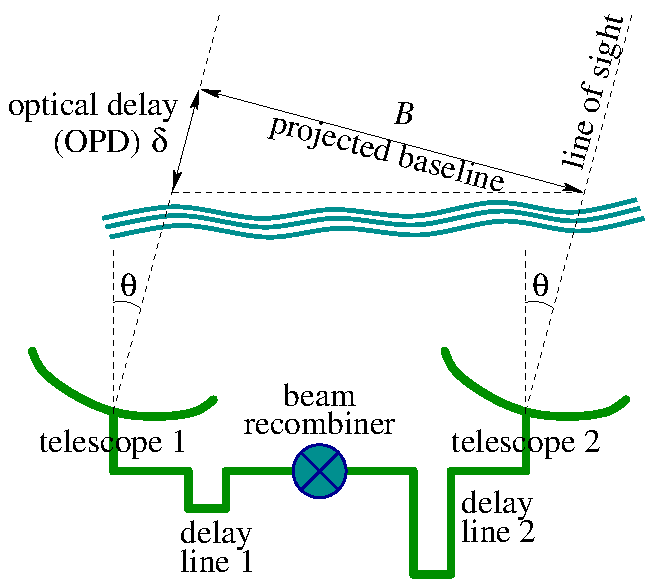
\includegraphics[width=60mm]{fig1}
  \caption{Geometrical layout of an interferometer. $B$ is the projected
    baseline, $\Dirn$ is the view angle and $\OPD$ is the geometrical optical
    path difference which is compensated by the delay lines.}
  \label{fig:layout}
\end{figure}

At short wavelengths (visible and infrared), the phase variance exceeds a few
squared radians and $\OTF_{j_1,j_2,m}\simeq0$, hence the object's complex
visibility cannot be directly measured.  A possible solution would be to
compensate for the OPD errors in real time using fast delay lines.  However,
this requires a bright reference source close to the observed object
and a \emph{dual-star} interferometer such as VLTI/PRIMA
\citep{Delplancke_at_al-2003-Prima} that can relate the phase measured on
the reference source to a simultaneous measurement of the target object. An
alternative approach is to integrate non-linear estimators that are
insensitive to telescope-wise phase errors.  This requires high acquisition
rates ($\sim1000\,\mathrm{Hz}$ in the near infrared) and involves special
data processing but otherwise no special instrumentation.

Following the second approach, most current optical interferometers integrate
the \vocab{power spectrum} (for $j_1\not=j_2$):
\begin{equation}
  \label{eq:mean-powerspectrum}
  \Powerspectrum_{j_1,j_2,m}
  = \avg{\abs{\ComplexVis_{j_1,j_2}(t)}^2}_m
  \simeq \GainSquaredModulus_{j_1,m} \,
         \GainSquaredModulus_{j_2,m} \,
         \abs{\FT{\Image}(\VFreq_{j_1,j_2,m})}^2 \,,
\end{equation}
with $\GainSquaredModulus_{j,m} = \avg{\abs{\Gain_{j}(t)}^2}_m$ the mean
squared modulus of the complex throughput of the $j$-th telescope during the
$m$-th exposure.  The transfer function $\GainSquaredModulus_{j_1,m} \,
\GainSquaredModulus_{j_2,m}$ of the power spectrum is insensitive to the phase
errors and can be estimated by simultaneous photometric calibration and, to
compensate for residual effects, from the power spectrum of a reference source
(a so-called \emph{calibrator}) observed shortly before and/or afterwards.
Hence measuring $\Powerspectrum_{j_1,j_2,m}$ gives the object power spectrum
$\abs{\FT{\Image}(\VFreq_{j_1,j_2,m})}^2$.

To obtain Fourier phase information, the \vocab{bispectrum} of the complex
visibilities is measured:
\begin{align}
  \Bispectrum_{j_1,j_2,j_3,m}
  &= \avg{\ComplexVis_{j_1,j_2}(t)\,\ComplexVis_{j_2,j_3}(t)\,
     \ComplexVis_{j_3,j_1}(t)}_m \notag \\
  &\simeq \GainSquaredModulus_{j_1,m} \,
     \GainSquaredModulus_{j_2,m} \,
     \GainSquaredModulus_{j_3,m} \,
     \FT{\Image}(\VFreq_{j_1,j_2,m}) \,
     \FT{\Image}(\VFreq_{j_2,j_3,m}) \,
     \FT{\Image}(\VFreq_{j_3,j_1,m}) \, , 
     \label{eq:mean-bispectrum}
\end{align}
where $j_1$, $j_2$ and $j_3$ denote three different telescopes.  As for the
power spectrum, the bispectrum transfer function $\GainSquaredModulus_{j_1,m}
\, \GainSquaredModulus_{j_2,m} \, \GainSquaredModulus_{j_3,m}$ can be
calibrated.  Since this transfer function is real, it has no effect on the
phase of the bispectrum (the so-called \vocab{closure phase}) which is equal to
that of the object.
% \begin{align}
%   \PhaseClosure_{j_1,j_2,j_3,m}
%   &\equiv \arg(\Bispectrum_{j_1,j_2,j_3,m}) \notag \\
%   &= \arg(\FT{\Image}(\VFreq_{j_1,j_2,m}) \,
%           \FT{\Image}(\VFreq_{j_2,j_3,m}) \,
%           \FT{\Image}(\VFreq_{j_3,j_1,m}))\, .
%   \label{eq:phase-closure}
% \end{align}
However a fraction of the phase information is missing.  The set of all
baselines between $T$ telescopes (in a non-redundant configuration), samples
$T\,(T - 1)/2$ different spatial frequencies but the closure phase only yields
$(T - 1)\,(T - 2)/2$ linearly independent phase
estimates~\citep{Monnier-2003-interferometry}.  The smaller the number of
telescopes, the larger the fraction of missing phase information.
Furthermore, all information on the absolute position of the observed object
is lost regardless of the number of telescopes.

In practice, obtaining the power spectrum and the bispectrum involves
measuring the instantaneous complex visibilities (that is, for a very short
integration time compared to the evolution of the turbulence) and averaging
their power spectrum and bispectrum over the effective exposure time.  Being
non-linear functions of noisy variables, these quantities are biased but the
biases are straightforward to remove \citep{Gordon_Buscher-2012-bias}.  To
simplify the description of the algorithms, we will consider that the
\emph{de-biased} and \emph{calibrated} power spectrum and bispectrum are
available as input data for image reconstruction, thus:
\begin{align}
  \Powerspectrum_{j_1,j_2,m}^\DataTag
  &= \abs{\FT{\Image}(\VFreq_{j_1,j_2,m})}^2
     + \Powerspectrum_{j_1,j_2,m}^\ErrorTag \, ,
  \label{eq:powerspectrum-data}
  \\
  \Bispectrum_{j_1,j_2,j_3,m}^\DataTag
  &= \FT{\Image}(\VFreq_{j_1,j_2,m}) \,
     \FT{\Image}(\VFreq_{j_2,j_3,m}) \,
     \FT{\Image}(\VFreq_{j_3,j_1,m}) \notag
     + \Bispectrum_{j_1,j_2,j_3,m}^\ErrorTag
  \label{eq:bispectrum-data}
\end{align}
where $\Powerspectrum_{j_1,j_2,m}^\ErrorTag$ and
$\Bispectrum_{j_1,j_2,j_3,m}^\ErrorTag$ are zero-mean terms that account for
noise and model errors.
% Instead of the complex bispectrum data, we may
% consider the closure phase data:
% \begin{align}
%   \PhaseClosure_{j_1,j_2,j_3,m}^\DataTag
%   &= \arc\bigl(\VisPhase(\VFreq_{j_1,j_2,m}) +
%           \VisPhase(\VFreq_{j_2,j_3,m}) \notag\\
%    &\hspace{4em}{+}\:\VisPhase(\VFreq_{j_3,j_1,m}) +
%         \PhaseClosure_{j_1,j_2,j_3,m}^\ErrorTag\bigr) \, ,
%   \label{eq:phase-closure-data}
% \end{align}
% where $\VisPhase(\VFreq)=\arg(\FT{\Image}(\VFreq))$ is the Fourier phase of
% the object brightness distribution, $\arc(\,)$ wraps its argument in the range
% $(-\pi,+\pi]$ and $\PhaseClosure_{j_1,j_2,j_3,m}^\ErrorTag$ denotes the
% errors.

%%%%%%%%%%%%%%%%%%%%%%%%%%%%%%%%%%%%%%%%%%%%%%%%%%%%%%%%%%%%%%%%%%%%%%%%%%%%%%%
%%%%%%%%%%%%%%%%%%%%%%%%%%%%%%%%%%%%%%%%%%%%%%%%%%%%%%%% IMAGE RECONSTRUCTION %
%%%%%%%%%%%%%%%%%%%%%%%%%%%%%%%%%%%%%%%%%%%%%%%%%%%%%%%%%%%%%%%%%%%%%%%%%%%%%%%

\section{Imaging from Sparse Fourier Data}
\label{sec:image-reconstruction}

We consider here the simplest problem of image reconstruction given sparse
Fourier coefficients (the complex visibilities), assuming that the OTF has
been calibrated. This discussion will inform the subsequent treatment of image
reconstruction from non-linear observables in
Sec.~\ref{sec:optical-interferometry}.

%==============================================================================
%====================================================== DATA AND IMAGE MODELS =
%==============================================================================

\subsection{Data and Image Models}
\label{sec:models}

To simplify the notation, we introduce the \emph{data vector}
$\Data\in\Complexes^L$ which collates all the complex visibility measurements:
$\Data[\ell]=\ComplexVis_{j_1,j_2,m}^\DataTag$ with $\ell\sim(j_1,j_2,m)$ to
denote a one-to-one mapping between index $\ell$ and triplet $(j_1,j_2,m)$.
Long baseline interferometers provide data for a limited set
$\FreqSet=\{\VFreq_k\}_{k=1,\ldots,K}$ of observed spatial frequencies,
corresponding to the projected baselines at the times of the observations.

% For each $\VFreq_k$, there is a non-empty set $\BaseSet_k$ of telescope pairs
% and exposures such that:
% \begin{displaymath}
%   (j_1,j_2,m) \in \BaseSet_k
%   \quad\Longleftrightarrow\quad
%   \VPosn_{j_2,m} - \VPosn_{j_1,m} = \Wavelength\,\VFreq_k
% \end{displaymath}
% or equivalently:
% \begin{equation}
%   \label{eq:base-set-def}
%   \BaseSet_k \bydef \left\{(j_1,j_2,m) \in \ApertureList^2\times\ExposureList
%   %\quad\text{s.t.}\quad
%   ;\ \VPosn_{j_2,m} - \VPosn_{j_1,m} = \Wavelength\,\VFreq_k \right\}
% \end{equation}
% with $\ApertureList$ and $\ExposureList$ the sets of apertures (telescopes or
% antennae) and exposure indexes, and $\VPosn_{j,m}=\avg{\VPosn_j(t)}_{m}$ the
% mean position of the $j$-th telescope during the $m$-th exposure.  Introducing
% $\BaseSet_k$ and the set $\FreqSet$ of observed frequencies is a simple way to
% account for all possible cases (with or without redundancies, multiple data
% sets, observations from different interferometers, \etc).  Note that, if every
% spatial frequency is only observed once, then $L=K$ and we can use $\ell=k$.

The image is a parametrized representation of the object brightness
distribution.  A very general description is given by a linear expansion:
\begin{equation}
  \label{eq:general-image-model}
  \Image(\VDirn) = \sum_{n=1}^{N} \Param_n \, \BasisFunc_n(\VDirn)
  \quad \stackrel{\mathrm{F.T.}}{\longrightarrow}\quad
  \FT{\Image}(\VFreq) = \sum_{n=1}^{N} \Param_n \, \FT{\BasisFunc}_n(\VFreq)
  \,,  
\end{equation}
where $\{\BasisFunc_n(\VDirn)\}_{n=1,\ldots,N}$ are basis functions and
$\VParam\in\Reals^N$ are the image parameters, for instance, the values of the
image \emph{pixels}, or wavelet coefficients.

% The function $\BasisFunc(\VDirn)$ can also be used as a \emph{building-block}
% for image reconstruction \citep{Hofmann_Weigelt-1993-building_blocks}.
% Alternatively, $\BasisFunc(\VDirn)$ may be seen as the \emph{neat beam} that
% sets the effective resolution of the image
% \citep{Lannes_et_al-1997-Clean_and_Wipe}.

The size of the synthesized field of view and the image resolution must be
chosen according to the extension of the observed object and to the resolution
of the interferometer.  To avoid biases and rough approximations caused by the
particular image model, the grid spacing $\Delta\Dirn$ should be well beyond
the limit imposed by the longest baseline:
\begin{equation}
  \label{eq:diffraction-limit}
  \Delta\Dirn \ll \frac{\lambda}{2\,\MaxBaseline}
\end{equation}
where $\MaxBaseline=\max_{j_1,j_2,t}\abs{\VPosn_{j_1}(t) - \VPosn_{j_2}(t)}$
is the maximum projected separation between interfering telescopes.
Oversampling by a factor of at least 2 is usually used, hence the pixel size is
given by: $\Delta\Dirn \lesssim \lambda/(4\,\MaxBaseline)$.  To avoid aliasing
and image truncation, the field of view must be chosen large enough and
without forgetting that the reciprocal of the width of the field of view also
sets the sampling step of the spatial frequencies.

The model of the complex visibility at the observed spatial frequencies is:
\begin{equation}
  \label{eq:sampled-image-FT}
  \ComplexVis_{k}(\VParam) = \FT{\Image}(\VFreq_k)
  = \sum_{n=1}^{N} \XForm[k,n] \, \Param_{n}
  \,,
\end{equation}
where the coefficients of the matrix $\XForm\in\Complexes^{K\times{}N}$ are
$\XForm[k,n] = \FT{\BasisFunc}_n(\VFreq_k)$.  The matrix $\XForm$ performs the
Fourier transform of non-equispaced data, which is a very costly operation.
This problem is not specific to interferometry, similar needs in
crystallography, tomography and bio-medical imaging have led to the
development of fast algorithms to approximate this operation
\citep{Potts_et_al-2001-NFFT_tutorial}.  For instance:
\begin{equation}
  \label{eq:Fourier-approximation}
  \XForm \simeq \InterpOp\cdot\DFTop\cdot\ApodizationOp \, ,
\end{equation}
where $\DFTop\in\Complexes^{N\times{}N}$ is the fast Fourier transform (FFT)
operator, $\InterpOp\in\Complexes^{K\times{}N}$ is a linear operator to
interpolate the discrete Fourier transform of the image
$\FT{\VParam}=\DFTop\cdot\VParam$ at the observed spatial frequencies and
$\ApodizationOp$ is diagonal and compensates the field of view apodization (or
spectral smoothing) caused by $\InterpOp$.

% In radio astronomy a different technique called \emph{regridding}
% \citep{Thompson_Bracewell-1974-Fourier_interpolation,1989ASPC....6..117X} is
% generally used, which consists in interpolating the data (not the model) onto
% the grid of discrete frequencies.  The advantage is that, when there is a
% large number of measurements, the number of data points is reduced, which
% speeds up further computations.  There are however a number of drawbacks to
% the regridding technique.  First it is not possible to apply the technique to
% non-linear estimators such as the power spectrum and the bispectrum.  Second,
% owing to the structure of the regridding operator, the regridded data are
% correlated even if the original data are not.  These correlations are usually
% ignored in further processing and the pseudo-data are assumed to be
% independent, which results in a poor approximation of the real noise
% statistics.  This can be a critical issue with low signal to noise data
% \citep{Meimon_et_al-2005-convex_approximation}.

Putting all this together, the direct model of the data is affine:
\begin{equation}
  \label{eq:Fourier-plane-data-model}
  \Data = \ModelOp\cdot\VParam + \Error
  %\quad\text{with\ }\ModelOp = \OTFop\cdot\XForm
\end{equation}
with $\Error$ the \emph{error vector}
($\Error[\ell]=\ComplexVis_{j_1,j_2,m}^\ErrorTag$), $\ModelOp =
\OTFop\cdot\XForm$ the linear model operator and 
$\OTFop\in\Complexes^{L\times{}K}$ the OTF operator given by:
\begin{equation}
  \label{eq:otf}
  \OTFop[\ell,k] = 
  \begin{cases}
     \Gain_{j_1,m}^{\star} \, \Gain_{j_2,m}^{}
     & \text{if } \ell\sim(j_1,j_2,m) \in \BaseSet_k\\[1ex]
     0 & \text{otherwise.}
  \end{cases}
\end{equation}
Here $\BaseSet_k$ is the set of telescope pairs and exposures yielding
spatial frequency $\VFreq_k$.

Applying the pseudo-inverse $\XForm^{+} =
\ApodizationOp^{-1}\cdot\DFTop^{-1}\cdot\InterpOp^{+}$ of $\XForm$ to the data
yields the so-called \emph{dirty image} (see \Fig{fig:dirty-map}):
\begin{equation}
  \label{eq:dirty-map}
  \mathring{\Data} = \XForm^{+}\cdot\Data = \M{H}\cdot\VParam
  + \mathring{\Error}
  %VParam_\Tag{dirty} = [\M{M}\T\cdot\Werror\cdot\M{M}]^{\dagger}
  %\cdot\M{M}\T\cdot\Werror\cdot\Data
\end{equation}
where $\mathring{\Error}=\XForm^{+}\cdot\Error$ and
$\M{H}=\XForm^{+}\cdot\OTFop\cdot\XForm$. Neglecting the apodization, $\M{H}$
essentially performs the convolution of the image by the \vocab{dirty beam}
(see \Fig{fig:dirty-map}).  From \Eq{eq:Fourier-plane-data-model} and
\Eq{eq:dirty-map}, image reconstruction from interferometric data can be seen
either as a problem of interpolating \emph{missing} Fourier coefficients or as
deconvolution of the dirty map by the dirty beam
\citep{Giovannelli_Coulais-2005-pos_mix}.

\begin{figure}[!t]
  \centering
  \begin{tabular}{lr}
  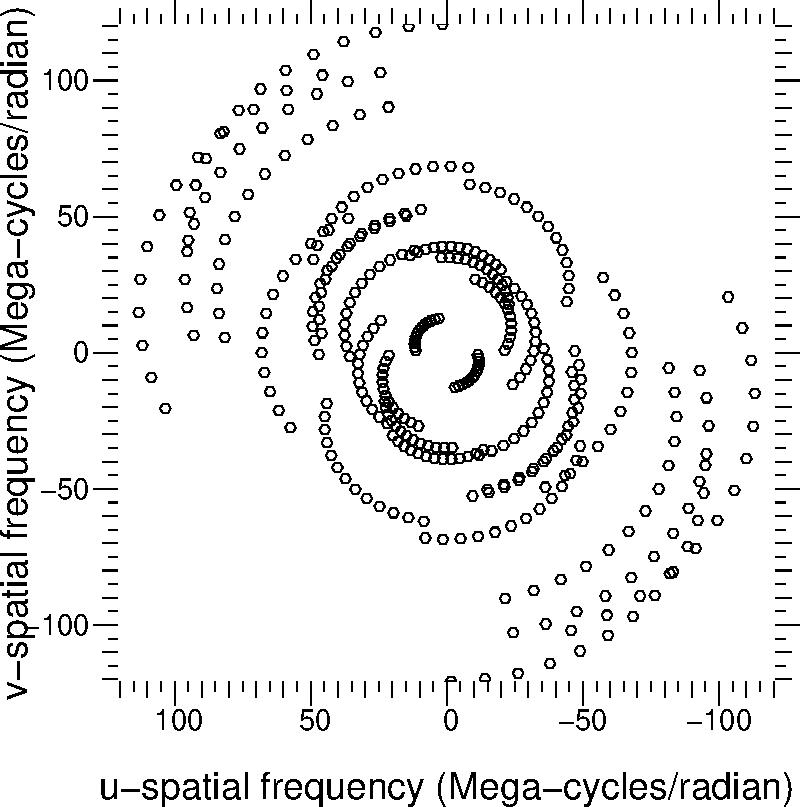
\includegraphics[height=30mm]{fig2a} &
  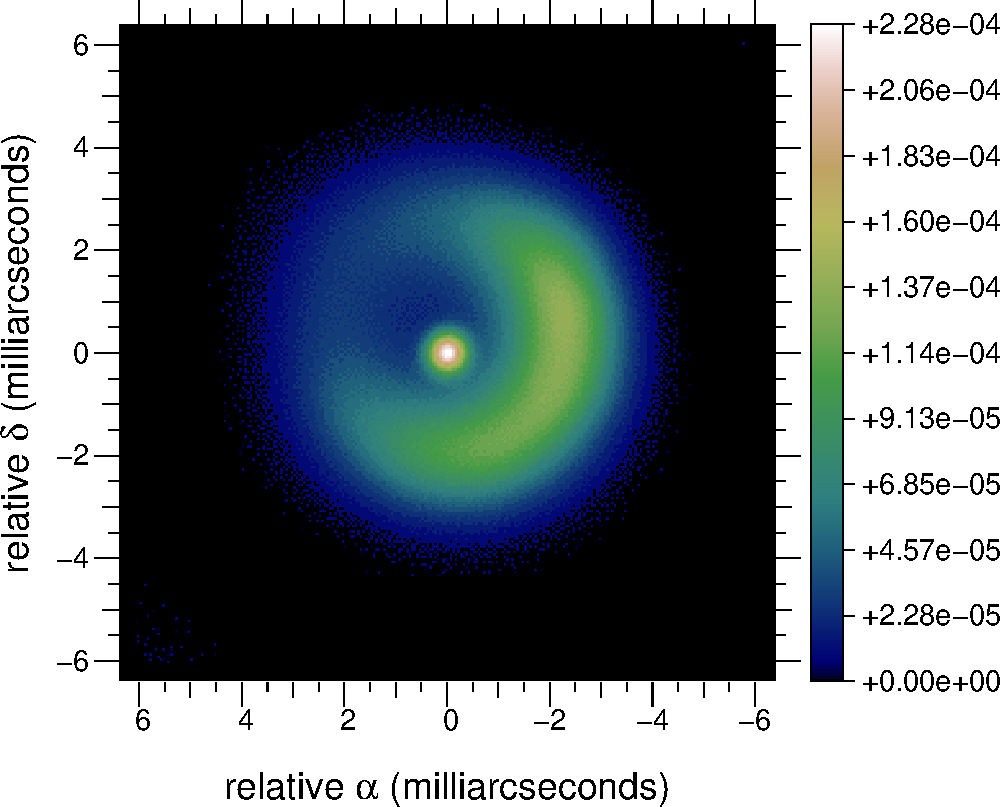
\includegraphics[height=30mm]{fig2b} \\[2mm]
  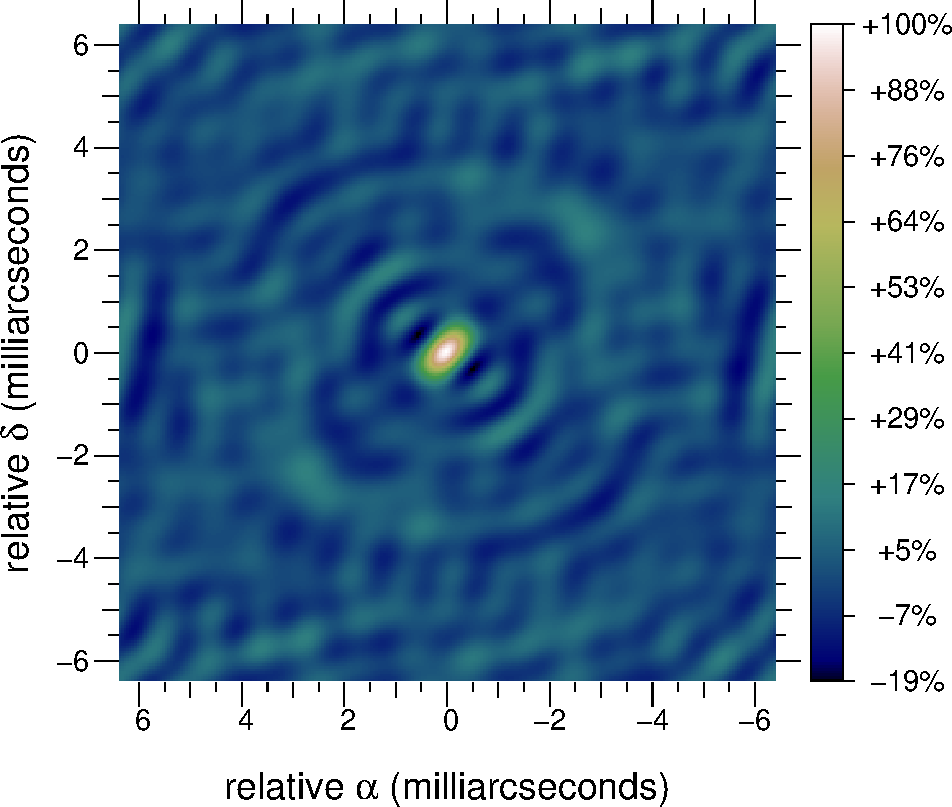
\includegraphics[height=30mm]{fig2c} &
  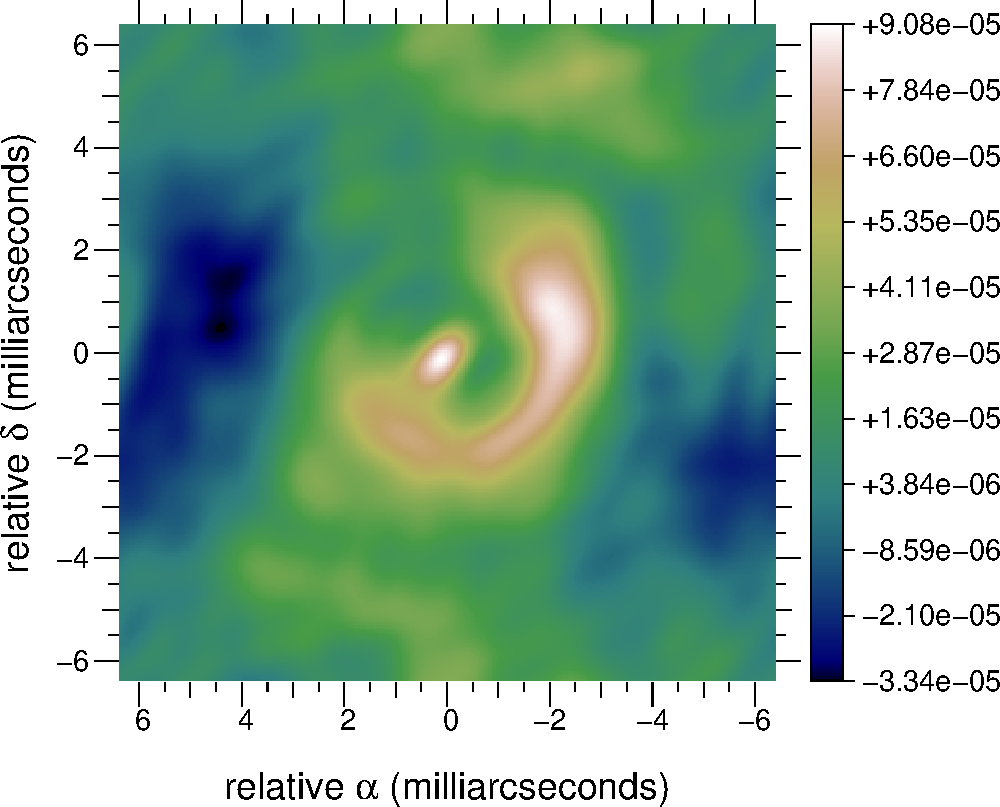
\includegraphics[height=30mm]{fig2d}\\
  \end{tabular}
  \caption{Top left: \uv coverage. Top right: observed object.  Bottom left:
    dirty beam.  Bottom right: dirty image.  Object model and \uv coverage are
    from the \emph{2004 Beauty Contest}
    \citep{beauty_contest-2004}.}
  \label{fig:dirty-map}
\end{figure}


%==============================================================================
%=========================================================== INVERSE APPROACH =
%==============================================================================

\subsection{Inverse Problem Approach}
\label{sec:inverse-approach}

Since many Fourier frequencies are not measured, simply fitting the data does
not uniquely define the desired image.  Such an ill-posed problem can be
solved by an inverse problem approach
\citep{Tarantola-2005-inverse_problem_theory} by imposing \apriori\
constraints to select a unique image among all those which are consistent with
the data.  The role of the priors is to smoothly interpolate voids in the \uv
coverage while avoiding high frequencies beyond the diffraction limit.
Without loss of generality, we assume that these constraints are monitored by
a penalty function $\Fprior(\VParam)$ which measures the agreement of the
image with the priors: the lower $\Fprior(\VParam)$, the better the agreement.
In the inverse problem framework, $\Fprior(\VParam)$ is known as the
\vocab{regularization}.  The parameters $\VParam^{+}$ of the image which
best matches the priors while fitting the data are obtained by solving a
constrained optimization problem:
\begin{equation}
  \label{eq:strict-data}
  \VParam^{+} = \argmin%_{\V{x}\in\FeasibleSet}
  \Fprior(\V{x}) \,,\ \text{subject to:\ }
  \ModelOp\cdot\VParam = \Data \, .
\end{equation}

Other strict constraints may apply.  For instance, assuming the image
brightness distribution must be positive and normalized, the feasible set is:
\begin{equation}
  \label{eq:feasible-set}
  \FeasibleSet =
  \{\VParam\in\Reals^N; \V{\Param} \ge 0, \sum_n \Param_n = 1\}
\end{equation}
where $\V{\Param} \ge 0$ means: $\forall n$, $\Param_n \ge 0$.  Rather than
enforce precise agreement with the data, we can instead measure the distance
of the model to the data by a penalty function $\Fdata(\VParam)$ and replace
the equality constraint in \Eq{eq:strict-data} with $\Fdata(\V{x}) \le
\DataLevel$. Here $\DataLevel$ is set according to the level of errors, in
order to avoid over-fitting the data:
\begin{equation}
  \label{eq:min-prior-st-data-const}
  \VParam^{+} = \argmin_{\VParam\in\FeasibleSet} \Fprior(\VParam)
  \,,\ \text{subject to:\ }
  \Fdata(\VParam) \le \DataLevel \, .
\end{equation}
The Lagrangian of this constrained optimization problem can be written as:
\begin{equation}
  \mathcal{L}(\VParam; \ell) = \Fprior(\VParam)
  + \ell\,\Bigl(\Fdata(\VParam) - \DataLevel\Bigr)
\end{equation}
where $\ell$ is the Lagrange multiplier associated with the inequality
constraint $\Fdata(\VParam)\le\DataLevel$.  If the constraint is
\emph{active}\footnote{Conversely, the constraint being \emph{inactive} would
  imply that $\ell=0$, which would mean that the data are useless, which is
  hopefully not the case...}, then $\ell>0$ and $\Fdata(\VParam)=\DataLevel$
\citep{Nocedal_Wright-2006-numerical_optimization}.  Dropping the constant
$\DataLevel$ which does not depend on $\VParam$, the solution is obtained by
solving either of the following problems:
\begin{align}
  \VParam^{+}
  &= \argmin_{\VParam\in\FeasibleSet}
     \{\Fprior(\VParam) + \ell\,\Fdata(\VParam)\} \notag \\
% &= \argmin_{\VParam\in\FeasibleSet}
%    \{\Fdata(\VParam) + \mu \, \Fprior(\VParam)\} \notag \\
  &= \argmin_{\VParam\in\FeasibleSet}
     \Fcost(\VParam; \mu) \, , \notag
\end{align}
where 
\begin{equation}
  \label{eq:cost-function}
  \Fcost(\VParam; \mu) = \Fdata(\VParam) + \mu \, \Fprior(\VParam)
\end{equation}
is the penalty function and the \vocab{hyperparameter} $\mu=1/\ell>0$ has to
be tuned to match the constraint $\Fdata(\VParam)=\DataLevel$.  Hence we can
equivalently consider that we are solving the problem of maximizing the
agreement of the model with the data subject to the constraint that the priors
be below a preset level:
\begin{equation}
  \label{eq:min-data-st-prior-const}
  \VParam^{+} = \argmin_{\VParam\in\FeasibleSet} \Fdata(\VParam)
  \,,\ \text{subject to:\ }
  \Fprior(\VParam) \le \PriorLevel \, .
\end{equation}
For convex penalties and providing that the Lagrange multipliers ($\mu$ and
$\ell$) and the thresholds ($\DataLevel$ and $\PriorLevel$) are set
consistently, image restoration is achieved by solving either of the
problems in \Eq{eq:min-prior-st-data-const}, \Eq{eq:min-data-st-prior-const}
or by minimizing the penalty function in \Eq{eq:cost-function}.  However,
choosing which of these particular problems to solve can be a deciding issue
for the efficiency of the method.  For instance, if $\Fdata(\VParam)$ and
$\Fprior(\VParam)$ are both \emph{smooth functions}, direct minimization of
$\Fcost(\VParam; \mu)$ in \Eq{eq:cost-function} can be done by using general
purpose optimization algorithms
\citep{Nocedal_Wright-2006-numerical_optimization}.

%==============================================================================
%======================================================= DISTANCE TO THE DATA =
%==============================================================================

\subsection{Distance to the Data}
\label{sec:fdata}

The $\ell_2$ norm is a simple means to measure the consistency of the model
image with the data:
\begin{equation}
  \label{eq:fdata-L2}
  \Fdata(\VParam) = \Norm{\Data - \ModelOp\cdot\VParam}^2_2\,.
\end{equation}
The distance to the data has to be defined according to the statistics of the
errors $\Error = \Data - \ModelOp\cdot\VParam$ given the image model.
Assuming Gaussian statistics, this leads to:
\begin{equation}
  \label{eq:fdata-Gaussian}
  \Fdata(\VParam) =
  \QuadTerm{\Werror}{(\Data - \ModelOp\cdot\VParam)} \,,
\end{equation}
where the weighting matrix $\Werror=\Cerror^{-1}$ is the inverse of the
covariance matrix of the errors.  There is a slight issue because we are
dealing with complex values.  Since complex numbers are just pairs of reals,
complex valued vectors (such as $\Data$, $\Error$ and $\ModelOp\cdot\VParam$)
can be \emph{flattened} into ordinary real vectors (with doubled size) to use
standard linear algebra notation and define the covariance matrix as
$\Cerror=\avg{\Error\cdot\Error\T}$.  This is what is assumed in
\Eq{eq:fdata-Gaussian}.

% There are some possible simplifications.  For instance, the complex
% visibilities are measured independently, hence the weighting matrix $\Werror$
% is block diagonal with $2\times2$ blocks.  Furthermore, if the real and
% imaginary parts of a given measured complex visibility are uncorrelated and
% have the same variance, then $\Fdata$ takes a simple form:
% \begin{equation}
%   \label{eq:fdata-Goodman}
%   \Fdata(\VParam) = \sum_\ell \Weight_{\ell} \,
%   \Abs{\Data[\ell] - (\ModelOp\cdot\VParam)_\ell}^2 \, ,
% \end{equation}
% where the weights are given by:
% \begin{equation}
%   \label{eq:fdata-Goodman-weights}
%   \Weight_{\ell}
%   = \Var\Paren{\Re\Paren{\Data[\ell]}}^{-1}
%   = \Var\Paren{\Im\Paren{\Data[\ell]}}^{-1} \, .
% \end{equation}
% This expression of $ \Fdata(\VParam)$, popularized by Goodman
% \citep{Goodman-statistical_optics}, is very commonly used in
% radio-interferometry.

Real data may however have different statistics.  For instance, the
\vocab{\OIFITS} exchange file format for optical interferometric data assumes
that the amplitude and the phase of complex data (complex visibility or
bispectrum) are independent \citep{Pauls_et_al-2005-oifits}. As a result, the
isocontours of the corresponding log-likelihood form a \emph{non-convex}
valley in the complex plane. \citet{Meimon_et_al-2005-convex_approximation}
have proposed quadratic convex approximations of the true log-likelihood and
have shown that their so-called \emph{local approximation} yields the best
results, notably when dealing with low signal to noise data.  For a complex
datum $\Data[\ell]=\rho_\ell\,\exp(\mathi\,\varphi_\ell)$, their local
quadratic approximation is written:
\begin{equation}
  \label{eq:fdata-local-approx}
  \Fdata(\VParam) = \sum_\ell \Brace{
    \frac{\Re\Paren{e_\ell\,\mathe^{-\mathi\,\varphi_\ell}}^2}
         {\sigma^2_{/\!/,\ell}}
    + \frac{\Im\Paren{e_\ell\,\mathe^{-\mathi\,\varphi_\ell}}^2}
           {\sigma^2_{\perp,\ell}}
  }
\end{equation}
where $\Error = \Data - \ModelOp\cdot\VParam$ denotes the complex residuals
and the variances parallel and perpendicular to the complex datum vector are:
\begin{equation}
  \sigma^2_{/\!/,\ell} = \Var(\rho_\ell) \, , \qquad
  \sigma^2_{\perp,\ell} = \rho_\ell^2\,\Var(\varphi_\ell) \, .
\end{equation}

%==============================================================================
%============================================================= Regularization =
%==============================================================================

\subsection{Regularization}
\label{sec:regularization}

Of all the methods for constraining the ill-posed imaging problem, maximum
entropy (MEM) has perhaps the longest history. MEM methods are based on the
1950s work of Jaynes on information theory; the underlying idea is to obtain
the least informative image which is consistent with the
data~\citep{Ables-1974-MEM}.  This amounts to minimizing a criterion like the
one in \Eq{eq:cost-function} with $\Fprior(\VParam) = -S(\VParam)$ where the
\vocab{entropy} $S(\VParam)$ measures the informational content of the image
$\VParam$.  In this framework, $\Fprior(\VParam)$ is sometimes called
\vocab{negentropy}.  Among all the expressions considered for the negentropy of
an image, one of the most popular is \citep{Gull_Skilling-1984-MEM}:
\begin{equation}
  \label{eq:mem-prior}
  \Fprior(\VParam) = \sum_n \left[
    \Param_n\,\log( \Param_n/\bar{\Param}_n) - \Param_n + \bar{\Param}_n
  \right]
\end{equation}
with $\bar{\VParam}$ the \vocab{default image}; that is, the one which would
be recovered in the absence of any data.  The default image $\bar{\VParam}$
can be taken as being a flat image, an image previously restored, an image of
the same object at a lower resolution, \etc\
% \citet{Narayan_Nityananda-1986-maximum_entropy_review} reviewed maximum
% entropy methods for radio-interferometry imaging and compared the other forms
% of the negentropy that have been proposed.  They argued that only
% non-quadratic priors can interpolate missing Fourier data and noted that such
% penalties also forbid negative pixel values.  The fact that there is no need
% to explicitly impose positivity is sometimes put forward by the proponents of
% these methods.
% MEM penalties are usually \emph{separable}, which means that they do not
% depend on the ordering of the pixels.  To explicitly enforce some correlation
% between close pixels in the sought image $\VParam$ (hence, some
% \emph{smoothness}), the prior can be chosen to depend on $\VParam$.  For
% instance: $\bar{\VParam}=\M{P}\cdot\VParam$ where $\M{P}$ is some averaging or
% smoothing linear operator.  This type of \emph{floating prior} has been used
% to loosely enforce constraints such as radial symmetry \citep{Horne1985}.
% Alternatively, an intrinsic correlation function (ICF) can be explicitly
% introduced by a convolution kernel to impose the correlation structure of the
% image~\citep{Gull-1989-MEM}.

Minimizing the joint criterion in \Eq{eq:cost-function} with entropy
regularization has a number of issues as the problem is highly non-linear and
the number of unknowns is very large (as many as there are pixels).
Various methods have been proposed, but the most effective algorithm
\citep{Skilling_Bryan-1984-maximum_entropy} employs non-linear optimization in
a local sub-space of search directions with the Lagrange multiplier $\mu$
tuned on the fly to match the constraint that $\Fdata(\VParam)=\DataLevel$.

Bayesian arguments can be invoked to define other types of regularization.
For instance, assuming that the pixels have a Gaussian distribution leads to
quadratic penalties such as:
\begin{equation}
  \label{eq:gauss-prior}
  \Fprior(\VParam) = \QuadTerm{\Cprior^{-1}}{(\VParam - \bar{\VParam})}
\end{equation}
with $\Cprior$ the prior covariance and $\bar{\VParam}$ the prior solution.
One simple but effective example is the \emph{compactness} penalty:
\begin{equation}
  \label{eq:fov-penalty}
  \Fprior(\VParam) = \sum_{n} w^\PriorTag_n\,\Param_n^2 \, ,  
\end{equation}
where the weights are increasing with the distance to the center of the image
thus favoring structures concentrated within this part of the image.  Under
strict normalization and positivity constraints and in the absence of any
data, the default image given by this prior is
$\bar{x}_n\propto1/w^\PriorTag_n$ where the factor comes from the
normalization requirement \citep{LeBesnerais_et_al-2008-interferometry}. This
regularizer is effective because imposing a compact, positive brightness
distribution gives rise to smooth interpolation in the Fourier plane.

Other prior penalties commonly used in image restoration methods can be useful
for interferometry.  For instance, \emph{edge-preserving smoothness} is
achieved by:
\begin{equation}
  \label{eq:edge-preserving-roughness}
  \Fprior(\VParam) = \sum_{n_1,n_2}
  \sqrt{\epsilon^2 + \abs{\nabla\VParam}_{n_1,n_2}^2}
\end{equation}
where $\epsilon>0$ is a chosen threshold and $\abs{\nabla\VParam}^2$ is the
squared magnitude of the spatial gradient of the image:
\begin{displaymath}
  \label{eq:spatial-gradient-magnitude}
  \abs{\nabla\VParam}_{n_1,n_2}^2 =
  (x_{n_1+1,n_2} - x_{n_1,n_2})^2 + (x_{n_1,n_2+1} - x_{n_1,n_2})^2 \, .
\end{displaymath}
The penalization in \Eq{eq:edge-preserving-roughness} behaves as a quadratic
function where the magnitude of the spatial gradient is small compared to
$\epsilon$, and a linear function when the gradient is large.  Hence reduction
of small local variations is achieved without over-penalizing strong sharp
features.  In the limit $\epsilon\rightarrow0$, edge-preserving smoothness
behaves like \emph{total variation} \citep{Rudin_et_al-1992-total_variation}
which has proved successful in imposing sparsity.

%%%%%%%%%%%%%%%%%%%%%%%%%%%%%%%%%%%%%%%%%%%%%%%%%%%%%%%%%%%%%%%%%%%%%%%%%%%%%%%
%%%%%%%%%%%%%%%%%%%%%%%%%%%%%%%%%%%%%%%%%%%%%%%%%%%%%% OPTICAL INTERFEROMETRY %
%%%%%%%%%%%%%%%%%%%%%%%%%%%%%%%%%%%%%%%%%%%%%%%%%%%%%%%%%%%%%%%%%%%%%%%%%%%%%%%

\section{Image Reconstruction from Non-Linear Data}
\label{sec:optical-interferometry}

At optical wavelengths, the complex visibilities are not directly measurable,
the available data (\cf\ Section \ref{sec:interferometric-data}) being the
power spectrum, the bispectrum and/or the closure phase.  Image reconstruction
algorithms that use these data can be designed to follow the same inverse
problem approach as above.  However, the direct model of the data is now
non-linear and specific expressions to implement $\Fdata$ have to be derived.
The non-linearity has also some impact on the optimization strategy.

\subsection{Data Penalty}

The power spectrum, the bispectrum, and the closure phase data have
non-Gaussian statistics: the power spectrum is a positive quantity, the
closure phase is wrapped in $(-\pi,+\pi]$, \etc\ However most algorithms use
penalties that are quadratic \wrt the measurements, which implies Gaussian
statistics in a Bayesian framework.  Another assumption generally made is the
independence of the measurements, which leads to \emph{separable} penalties.
Under such approximations, the penalty \wrt the power spectrum data is
written:
\begin{equation}
  \label{eq:powerspectrum-penalty}
  \Fdata^\PowerspectrumTag(\VParam) = \sum_{m, j_1 < j_2}
  \frac{  \Paren{\Powerspectrum_{j_1,j_2,m}^\DataTag
   - \Powerspectrum_{j_1,j_2,m}^\ModelTag(\VParam)}^2
  }{\Var\Paren{\Powerspectrum_{j_1,j_2,m}^\DataTag}} \, ,
\end{equation}
with $\Powerspectrum_{j_1,j_2,m}^\ModelTag(\VParam) =
\abs{\FT{\Image}(\VFreq_{j_1,j_2,m})}^2$ the model of the power spectrum.  For
the penalty \wrt the bispectrum data, there is the additional difficulty
of dealing with complex data.  The Goodman approximation
\citep{Goodman-statistical_optics} yields:
\begin{equation}
  \label{eq:bispectrum-penalty}
  \Fdata^\BispectrumTag(\VParam) =
  \hspace{-1em}\sum_{m, j_1 < j_2 < j_3}\hspace{-1em}
  w^\BispectrumTag_{j_1,j_2,j_3,m}\,
  \Abs{\Bispectrum_{j_1,j_2,j_3,m}^\DataTag
   - \Bispectrum_{j_1,j_2,j_3,m}^\ModelTag(\VParam)}^2
\end{equation}
with $\Bispectrum_{j_1,j_2,j_3,m}^\ModelTag(\VParam) =
\FT{\Image}(\VFreq_{j_1,j_2,m}) \, \FT{\Image}(\VFreq_{j_2,j_3,m}) \,
\FT{\Image}(\VFreq_{j_3,j_1,m})$ the model of the bispectrum and the weights
are derived from the variance of the bispectrum data.  An expression similar
to that in \Eq{eq:fdata-local-approx} can be derived for bispectrum data with
independent modulus and phase errors~\citep{Meimon_et_al-2009-selfcal}.  To
account for phase wrapping, \citet{Haniff1991} proposed to define the penalty
\wrt the closure phase data as:
\begin{equation}
  \label{eq:Haniff-phase-closure-penalty}
  \Fdata^\PhaseClosureTag(\VParam) =
  \hspace{-1em}\sum_{m, j_1 < j_2 < j_3}\hspace{-1em}
  \frac{
    \arc^2\Paren{\PhaseClosure_{j_1,j_2,j_3,m}^\DataTag
   - \PhaseClosure_{j_1,j_2,j_3,m}^\ModelTag(\VParam)}
  }{\Var\Paren{\PhaseClosure_{j_1,j_2,j_3,m}^\DataTag}}
\end{equation}
with $\PhaseClosure_{j_1,j_2,j_3,m}^\ModelTag(\VParam) =
\VisPhase(\VFreq_{j_1,j_2,m}) + \VisPhase(\VFreq_{j_2,j_3,m}) +
\VisPhase(\VFreq_{j_3,j_1,m})$ the model of the closure phase.  However, this
penalty is not continuously differentiable \wrt $\VParam$, which can prevent
the convergence of optimization algorithms.  This problem can be avoided by
using the complex phasors \citep{Thiebaut-2008-Marseille}:
\begin{equation}
  \label{eq:Mira-phase-closure-penalty}
  \Fdata^\PhaseClosureTag(\VParam) =
  \hspace{-1em}\sum_{m, j_1 < j_2 < j_3}\hspace{-1em}
  \frac{
    \bigl\vert
      \mathe^{\mathi\,\PhaseClosure_{j_1,j_2,j_3,m}^\DataTag}
    - \mathe^{\mathi\,\PhaseClosure_{j_1,j_2,j_3,m}^\ModelTag(\VParam)}
    \bigr\vert^2
  }{\Var\Paren{\PhaseClosure_{j_1,j_2,j_3,m}^\DataTag}} \, ,
\end{equation}
which is approximately equal to the penalty in
\Eq{eq:Haniff-phase-closure-penalty} in the limit of small closure phase
errors.

Depending on which types of data are available, and assuming that the
different types of data have statistically independent errors, the
\emph{total} penalty \wrt the data is simply a sum of some of the penalties
given by
equations~(\ref{eq:powerspectrum-penalty})--(\ref{eq:Mira-phase-closure-penalty}).
For instance, to fit the power spectrum and the closure phase data:
\begin{equation}
  \Fdata(\VParam) = \Fdata^\PowerspectrumTag(\VParam) +
  \Fdata^\PhaseClosureTag(\VParam) \, .
\end{equation}


\subsection{Image Reconstruction Algorithms}
\label{sec:new-methods}

We now describe the image reconstruction methods that have been successful on
realistic optical interferometric data and which are sufficiently mature to be
used with real data.  In addition to coping with sparse Fourier data, these
methods were specifically designed to tackle the non-linear direct model, to
account for the particular statistics of the data
\citep{Meimon_et_al-2005-convex_approximation} and to handle the new data
format \citep{Pauls_et_al-2005-oifits}. A summary of the methods is given in
\Tab{tab:algorithms}.

\begin{table}
  \begin{center}
    \begin{tabular}{p{6.2em}p{7.8em}p{8.9em}l}
      \hline
      \hline
      Name & Authors & Optimization & Regularization \\
      \hline
      BSMEM & Baron, Buscher & Trust region gradient & MEM-prior \\
      MiRA & Thi{\'e}baut & VMLM-B$^{(\star)}$ & Many \\
      WISARD & Meimon, Mugnier, Le~Besnerais &  VMLM-B$^{(\star)}$ plus self-calibration & Many \\
      \hline
      MACIM & Ireland, Monnier & Simulated annealing & MEM \\
      SQUEEZE & Baron, Monnier, Kloppenborg & Parallel tempering & \\
      \hline
      Building Block method & Hofmann, Weigelt & Matching pursuit & Sparsity \\
      \hline
      \hline
    \end{tabular}
  \end{center}
  \caption{\label{tab:algorithms} Summary of the algorithms for image
    reconstruction from optical interferometric data described in
    Section~\ref{sec:new-methods}.
    %\\$^{(\star)}$ VMLM-B is a quasi-Newton method with bounds
    % on the parameters
    %\citep{Thiebaut-2002-optim_bdec}
   }
\end{table}

\textit{1) BSMEM} algorithm \citep{Buscher-1994-BSMEM,
  Baron_Young-2008-Marseille} makes use of a Maximum Entropy Method
(Section~\ref{sec:regularization}) to regularize the problem of image
restoration from the measured bispectrum (hence its name).  The improved BSMEM
version \citep{Baron_Young-2008-Marseille} uses the Gull and Skilling entropy,
see \Eq{eq:mem-prior}, and a likelihood term with respect to the complex
bispectrum which assumes independent Gaussian noise statistics for the
amplitude and phase of the measured bispectrum.  The optimization engine is
\textsc{MemSys} which implements the strategy proposed by
\citet{Skilling_Bryan-1984-maximum_entropy} and automatically finds the most
likely value for the hyperparameter $\mu$. Because it makes no attempt to
directly convert the data into complex visibilities, a strength of \BSMEM is
that it can handle any type of data sparsity (such as missing closure phases).


\textit{2) The Building Block Method}
\citep{Hofmann_Weigelt-1993-building_blocks} is similar to the CLEAN method
but designed for reconstructing images from bispectrum data obtained by means
of speckle or long baseline interferometry.  The method proceeds iteratively
to reduce a cost function $\Fdata^\BispectrumTag$ equal to that in
\Eq{eq:bispectrum-penalty} with weights set to a constant or to an expression
motivated by Wiener filtering.  The minimization of the penalty is achieved by
a matching pursuit algorithm which imposes sparsity of the solution.  The
image is given by the building block model in \Eq{eq:general-image-model} and,
at the $n$-th iteration, the new image $\Image^{[n]}(\VDirn)$ is obtained by
adding a new building block at location $\VDirn^{[n]}$ with a weight
$\alpha^{[n]}$ to the previous image, so as to maintain the normalization:
\begin{displaymath}
  %\label{eq:building-block-next-image-normalized}
  \Image^{[n]}(\VDirn)
   = (1 - \alpha^{[n]})\,\Image^{[n - 1]}(\VDirn)
  + \alpha^{[n]} \, \BasisFunc(\VDirn - \VDirn^{[n]}) \, .\notag
\end{displaymath}
The weight and location of the new building block is derived by minimizing the
criterion $\Fdata^\BispectrumTag$ \wrt these parameters.  Strict positivity
and support constraints can be trivially enforced by limiting the possible
values for $\alpha^{[n]}$ and $\VDirn^{[n]}$. To avoid super
resolution artifacts, the final image is convolved with a smoothing function
with size set according to the spatial resolution of the instrument.

%\begin{align}
%  %\label{eq:building-block-next-image}
%  \Image^{[n]}(\VDirn)
%  & = \Image^{[n - 1]}(\VDirn)
%     + \alpha^{[n]} \, \BasisFunc(\VDirn - \VDirn^{[n]}) \notag\\
%\intertext{or, if strict normalization is applied:}
%  %\label{eq:building-block-next-image-normalized}
%  \Image^{[n]}(\VDirn)
%  & = (1 - \alpha^{[n]})\,\Image^{[n - 1]}(\VDirn)
%  + \alpha^{[n]} \, \BasisFunc(\VDirn - \VDirn^{[n]}) \, .\notag
%\end{align}

\textit{3) \Macim algorithm} \citep{Ireland_et_al-2006-MACIM}, for MArkov Chain
IMager, aims at maximizing the posterior probability:
\begin{displaymath}
  \Pr(\VParam\vert\Data)\propto
  \exp\Bigl(-\frac{1}{2}\,\Fdata(\VParam)
  - \frac{\mu}{2}\,\Fprior(\VParam)\Bigr) \,.
\end{displaymath}
\Macim implements MEM regularization and a specific regularizer which favors
large regions of dark space in between bright regions.  For this latter
regularization, $\Fprior(\VParam)$ is the sum of all pixels with zero flux on
either side of their boundaries.  \Macim attempts to maximize
$\Pr(\VParam\vert\Data)$ by a simulated annealing algorithm with the
Metropolis sampler.  Although maximizing $\Pr(\VParam\vert\Data)$ is the same
as minimizing $\Fdata(\VParam)+\mu\,\Fprior(\VParam)$, the use of
\emph{normalized} probabilities is required by the Metropolis sampler to
accept or reject the image samples. Simulated annealing can in principle solve
the global optimization problem of maximizing $\Pr(\VParam\vert\Data)$, but
convergence can be very slow, especially for objects comprising multiple
components.

\textit{4) \Squeeze algorithm} \citep{Baron_et_al-2010-SQUEEZE} was developed
recently by Fabien Baron and John Monnier at the University of Michigan, with
the collaboration of Brian Kloppenborg from the University of Denver. \Squeeze
has a very comprehensive set of features, including both Markov Chain Monte
Carlo (as in \Macim) and gradient-based optimization engines, and the ability
to combine geometric model-fitting with model-independent imaging. Novel
capabilities such as wavelet regularization within the compressed sensing
framework and imaging on spheroids are also being implemented.

\textit{5) \Mira algorithm} \citep{Thiebaut-2008-Marseille} defines the sought
image as the minimum of the penalty function in \Eq{eq:cost-function}.
Minimization is done by a limited variable memory method (based on BFGS
updates) with bound constraints for the positivity
\citep{Thiebaut:spie2002:bdec}.  \Mira is written in a modular way: any type
of data can be taken into account by providing a function that computes the
corresponding penalty and its gradient.  For the moment, \Mira handles complex
visibility, power spectrum and closure-phase data via penalty terms given by
\Eq{eq:fdata-local-approx}, \Eq{eq:powerspectrum-penalty} and
\Eq{eq:Mira-phase-closure-penalty}. \Mira can cope with any missing data, in
particular, it can be used to restore an image given only the power spectrum
(\ie\ without any Fourier phase information) with at least a $180^\circ$
orientation ambiguity.

\textit{6) \Wisard algorithm} \citep{Meimon_et_al-2005-weak_phase_imaging}
recovers an image from power spectrum and closure phase data.  It exploits a
self-calibration approach
\citep{Readhead_Wilkinson-1978-VLBI,Cornwell_Wilkinson-1981-self_calibration}
to recover missing Fourier phases.  Given a current estimate of the image and
the closure phase data, \Wisard first derives missing Fourier phase
information in such a way as to minimize the number of unknowns.  Then, the
synthesized Fourier phases are combined with the square root of the measured
power spectrum to generate pseudo complex visibility data which are fitted by
the image restoration step.  This step is performed by using the chosen
regularization and a penalty with respect to the pseudo complex visibility
data. This approach gives a unique solution for the image restoration step,
although overall the global problem remains multi-modal.

\Mira and \Wisard have been developed in parallel and share some common
features.  They use the same optimization engine
\citep{Thiebaut:spie2002:bdec} and means to impose positivity and
normalization \citep{LeBesnerais_et_al-2008-interferometry}.  However they
differ in the way missing data is taken into account: \Wisard
\emph{explicitly} solves for missing Fourier phase information; while \Mira
\emph{implicitly} accounts for any lack of information through the direct
model of the data~\citep{LeBesnerais_et_al-2008-interferometry}. Both implement
many different regularizers (negentropy, quadratic or edge-preserving
smoothness, compactness, total variation, \etc)

\subsection{Image Reconstruction Inputs}
\label{sec:inputs}

\subsubsection{\OIFITS data}

The algorithms described in Sec.~\ref{sec:new-methods} all accept data in the
form of one or more \OIFITS files. \OIFITS~\citep{Pauls_et_al-2005-oifits} is
a registered convention based on the FITS
standard~\citep{Hanisch_et_al-2001-fits}, designed for storage of calibrated
optical interferometric data. Supplementing the formal definition of \OIFITS,
\citet{Pauls_et_al-2004-oifits-spie} give an overview of the convention and
explains the design decisions taken.

An \OIFITS file can store data for multiple observing targets, taken with
multiple interferometers/instruments. The supported observables are the
complex visibility, power spectrum (squared visibility in \OIFITS parlance)
and bispectrum (triple product). The bispectrum phase (closure phase) may be
stored without a corresponding bispectrum amplitude. Each observable is stored
in a separate type of table, and any number of (including zero) instances of
each table type may be present in the file. Telescope (station) identifiers,
observation times and wavebands (wavelength and spectral bandwidth) are also
stored, the latter in separate tables to reduce duplication.

The typical steps involved in reading a set of \OIFITS files for image
reconstruction are as follows:
\begin{itemize}
\item Merge multiple \OIFITS files specified by the user

\item Extract data for the observing target, timespan and wavelengths
  (specified as a numerical range or set of \verb+INSNAME+ values) specified
  by the user

\item Determine the observation times and wavelengths of all usable data
  (usable meaning not flagged and comprising an appropriate combination of
  observables, for example powerspectra and bispectra measured simultaneously
  using the same telescopes and spectral channels)

\item Extract the usable data for these observation times and wavelengths
\end{itemize}

Proposals for extending \OIFITS have been discussed at length by the
community, and we expect that preliminary versions of these extensions will be
agreed in the near future, so that they can be used in preparing the test
datasets for the JRA. The planned extensions include conventions for storing
wavelength-differential visibility data and the spectral energy distribution
of the observed object. Wherever possible, the test datasets should also
validate as standard OIFITS.

\subsubsection{Image model parameters}

The most common pixellated image model comprises a shift-invariant set of
basis functions $\BasisFunc_n(\VDirn) = \BasisFunc(\VDirn - \VDirn_n)$ on an
equispaced two-dimensional grid $\{\VDirn_n\}$, with $\BasisFunc(\VDirn)$ the
pixel shape.

The pixellated model is usually parametrised by the grid spacing $\Delta\Dirn$
and the field of view given by the overall extent of the grid. As mentioned in
Sec.~\ref{sec:models}, the grid spacing must oversample the diffraction limit
by a sufficient factor to avoid modeling errors, bearing in mind that a degree
of super-resolution in the reconstructed image can often be achieved. The
field of view must be large enough to avoid aliasing. Often the precise size
of the observed object is unknown, so the image size would be chosen based on
the instrumental field of view. It is quite feasible to choose the image model
parameters automatically based on the range of spatial frequencies in the data,
perhaps rounding $\Delta\Dirn$ to a few significant figures.

\subsubsection{Regularization parameters}

A summary of the regularization types implemented by \Mira, \Wisard and \BSMEM
is given in \Tab{tab:regularization}. \citet{Renard-2011-regularization}
compared these regularization methods plus several others. As expected they
concluded that the best prior depends on the object of interest.  However,
edge-preserving smoothness (\Eq{eq:edge-preserving-roughness}), and
compactness (\Eq{eq:fov-penalty}) were shown to be successful in most
cases. Astronomers should not attach too much importance to the choice of
regularizer: Figure~\ref{fig:regularization-types} shows image reconstructions
using different types of regularization, all of which are fairly similar and
acceptable for publication.

The MEM-prior regularization involves a prior model, the \vocab{default
  image}. An informative prior model can be useful for constraining the
reconstruction when the data are sparse or noisy, otherwise it just speeds up
convergence. If the data consist of only powerspectra and/or bispectra, the
position of the object is completely unconstrained --- a non-flat default
image can be used to fix the position. For other priors, a non-flat initial
model used to start the optimization will serve the same purpose.

Irrespective of the particular form of $\Fprior(\VParam)$, the degree of
regularization imposed is set by the value of the hyperparameter $\mu$ in
\Eq{eq:cost-function}. This should strictly be derived from Bayesian
considerations but can be done quite accurately by visual inspection of the
restored image.  From \Fig{fig:regularization-levels}, one can see the effects
of under-regularization (which yields more artifacts) and over-regularization
(which yields over-simplification of the image).

\begin{table}
  \begin{center}
    {\small
    \begin{tabular}{p{8em}lll}
      \hline
      \hline
      Name & $\Fprior(\VParam)$ & Parameters & Implemented by \\
      \hline
      Quadratic smoothness
      & $\norm{\VParam - \V{S} \cdot \VParam}^2$ & & \Mira, \Wisard? \\
      \hline
      MEM-sqrt & $-\sum_n \sqrt{\Param_n} $ & & \Mira \\
      MEM-log  & $-\sum_n \log( \Param_n ) $ & & \Mira \\
      MEM-prior
      & $\sum_n \left[
        \Param_n\,\log( \Param_n/\bar{\Param}_n) - \Param_n + \bar{\Param}_n
      \right]$
      & Default image $\bar{\VParam}$ & \Mira, \BSMEM \\
      \hline
      Compactness
      & $\sum_n w^\PriorTag_n\,\Param_n^2; \,
      w^\PriorTag_n = \norm{\VDirn_n}^\beta$ & $\beta$ & \Mira \\
      \hline
      Edge-preserving smoothness
      $\epsilon\!\rightarrow\!0\implies\text{TV}$
      & $\sum_{n_1,n_2}\sqrt{\epsilon^2 + \abs{\nabla\VParam}_{n_1,n_2}^2}$
      & $\epsilon$ & \Mira, \Wisard \\
      \hline
      \hline
    \end{tabular}
  }
  \end{center}
  \caption{\label{tab:regularization} Summary of the most useful
    regularization types implemented by the algorithms being developed under
    the JRA. The names used here are taken from
    \citet{Renard-2011-regularization}.
  }
\end{table}

\begin{figure}[!t]
  \centering
  \begin{tabular}{lcr}
  &
  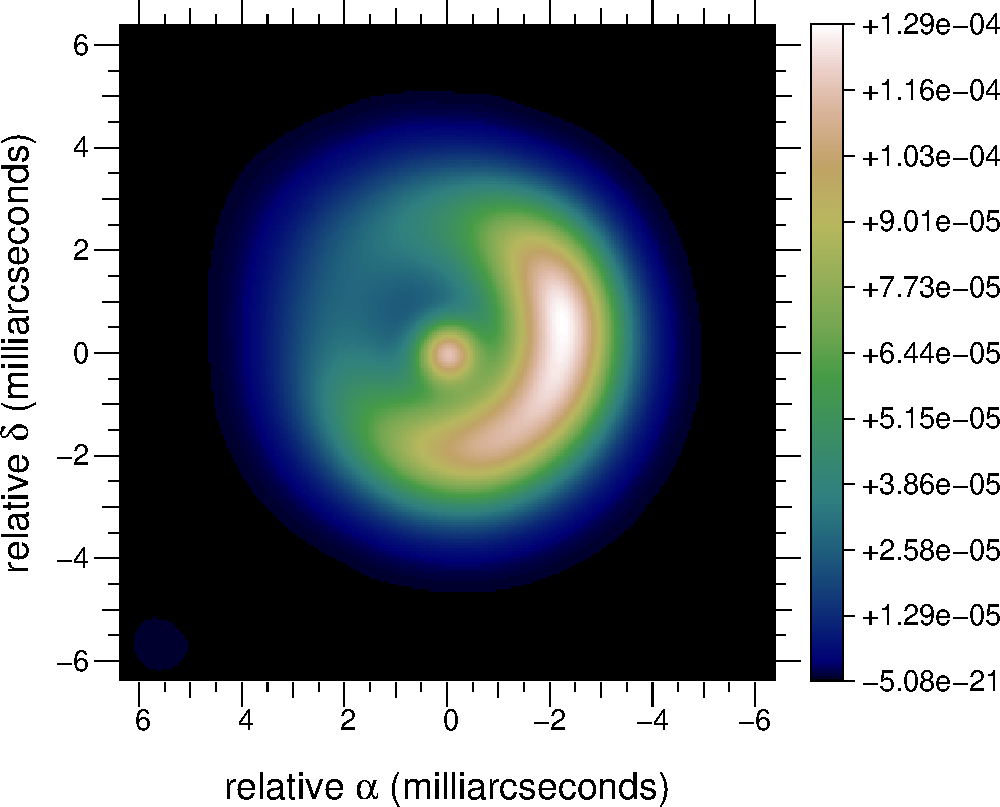
\includegraphics[height=30mm]{fig3a} &
  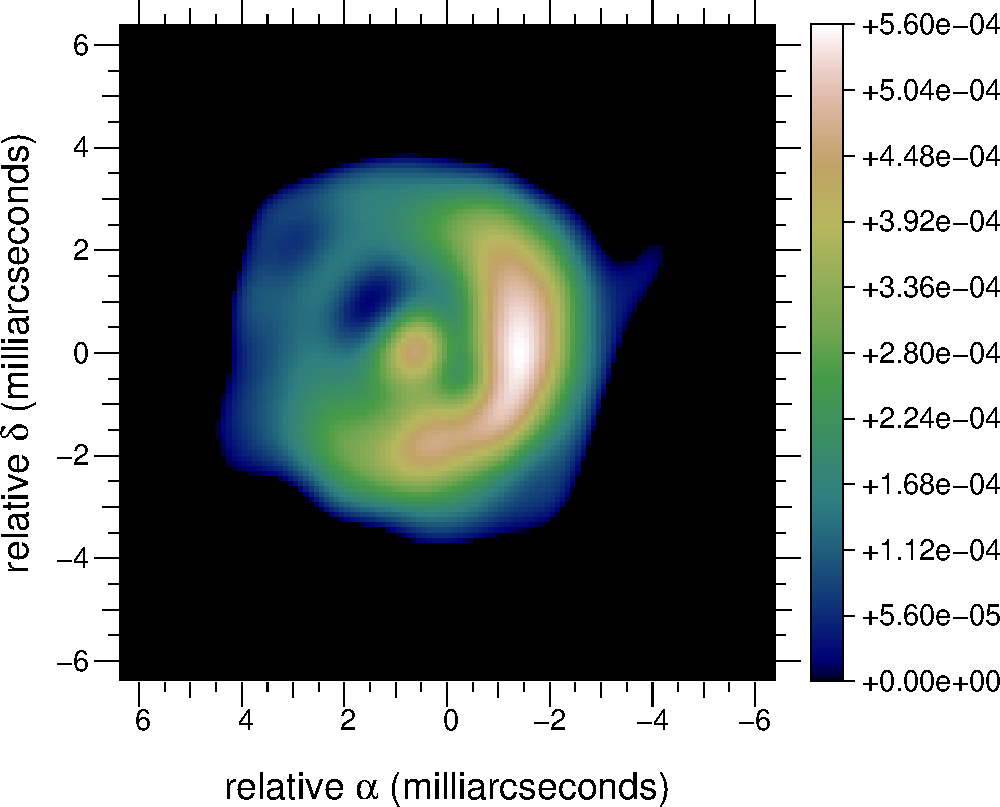
\includegraphics[height=30mm]{fig3b} \\[2mm]
  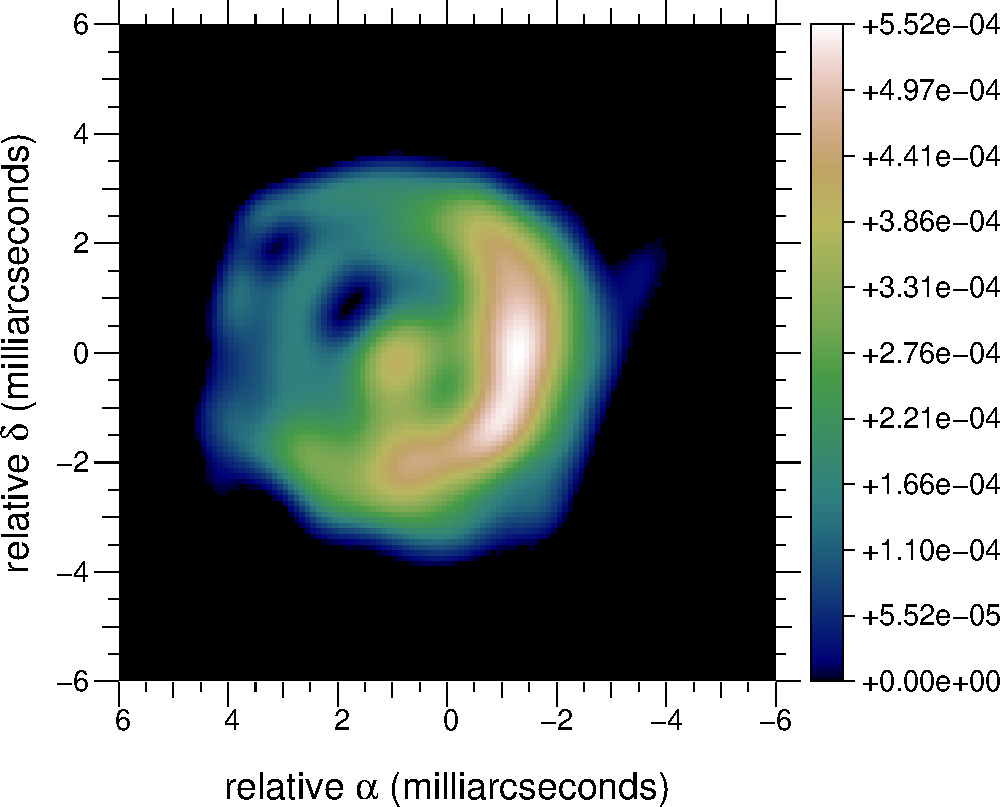
\includegraphics[height=30mm]{fig3c} &
  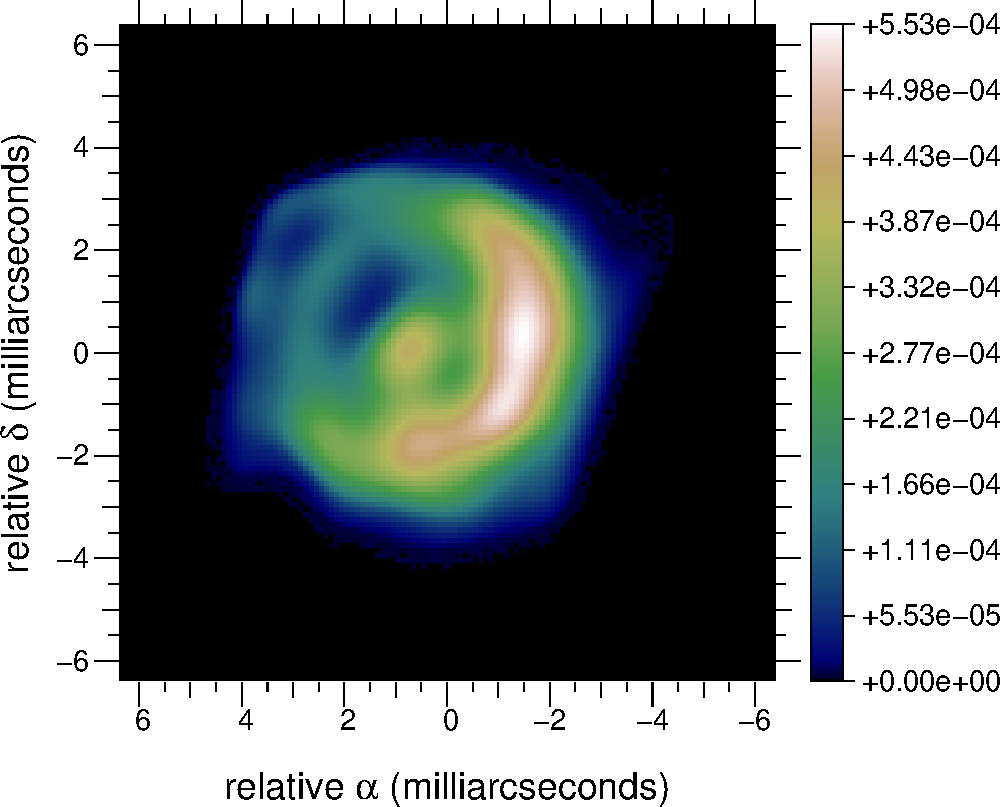
\includegraphics[height=30mm]{fig3d} &
  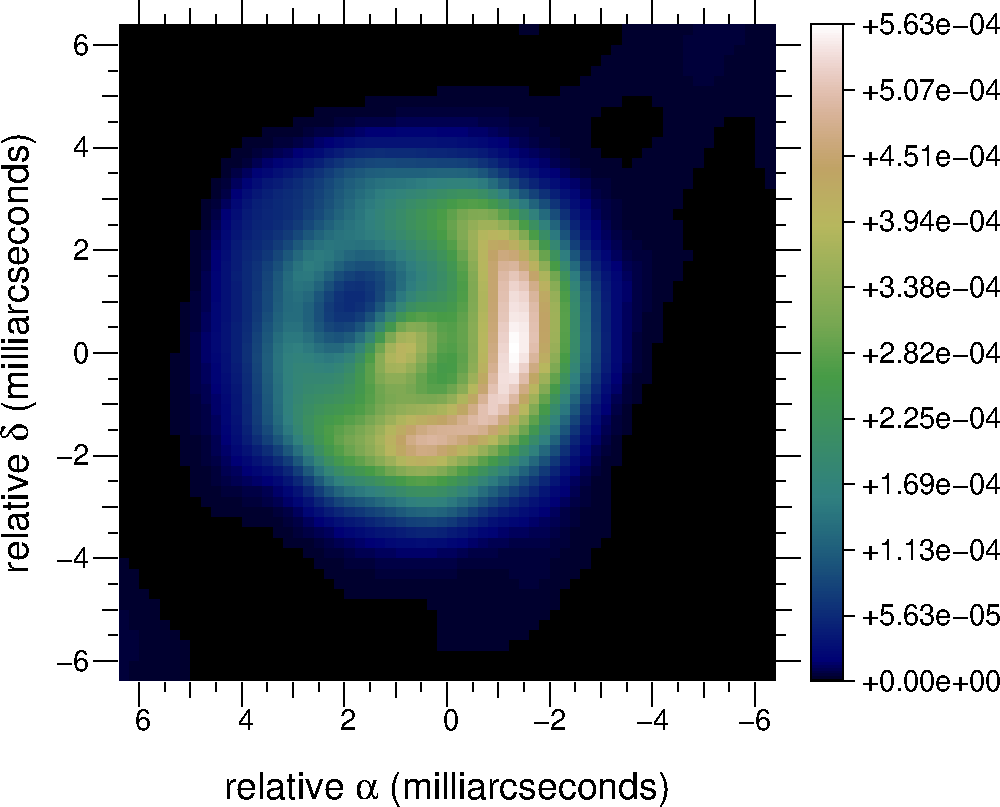
\includegraphics[height=30mm]{fig3e-alt}\\
  \end{tabular}
  \caption{\Mira and \BSMEM image reconstructions with various types of
    regularization.  From top-left to bottom-right: (a) original object
    smoothed to the resolution of the interferometer
    ($\mathrm{FWHM}\sim15\,\mathrm{mas}$); (b) \Mira reconstruction with a
    compactness quadratic regularization given by
    Eq.~(\protect\ref{eq:fov-penalty}); (c) \Mira reconstruction with
    edge-preserving regularization as in
    Eq.~(\protect\ref{eq:edge-preserving-roughness}); (d) \Mira reconstruction
    with MEM regularization as in Eq.~(\protect\ref{eq:mem-prior}); (e) \BSMEM
    reconstruction with MEM regularization.}
  \label{fig:regularization-types}
\end{figure}


\begin{figure}[!t]
  \centering
  \begin{tabular}{lr}
  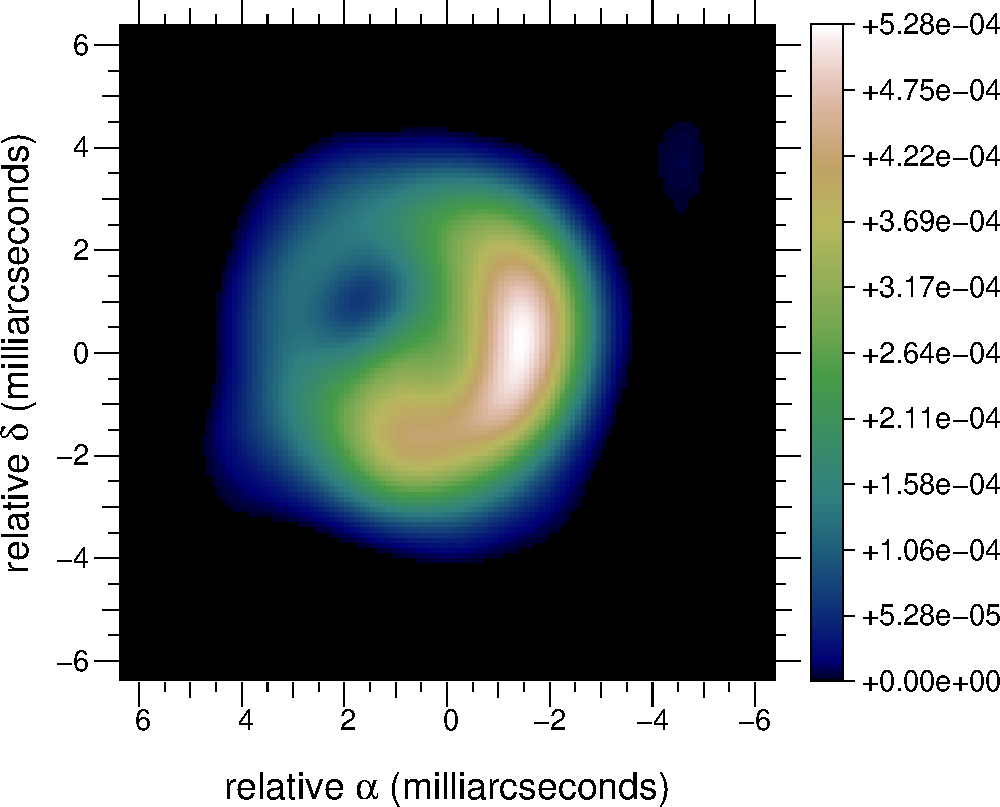
\includegraphics[height=30mm]{fig4a} &
  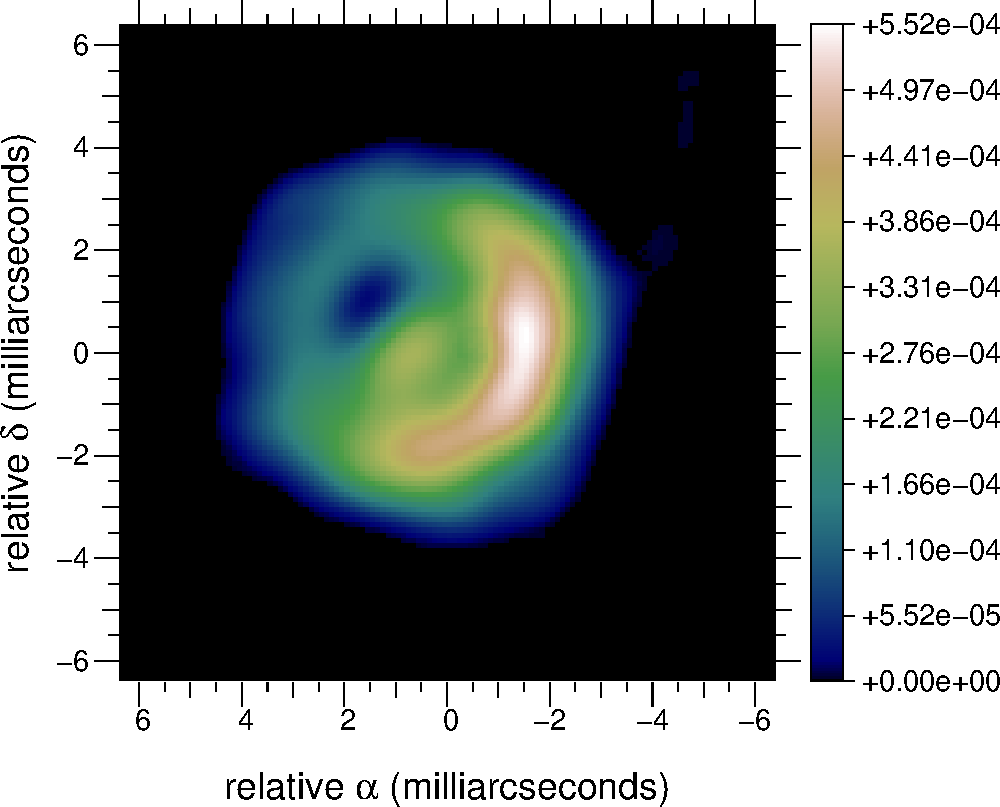
\includegraphics[height=30mm]{fig4b} \\[2mm]
  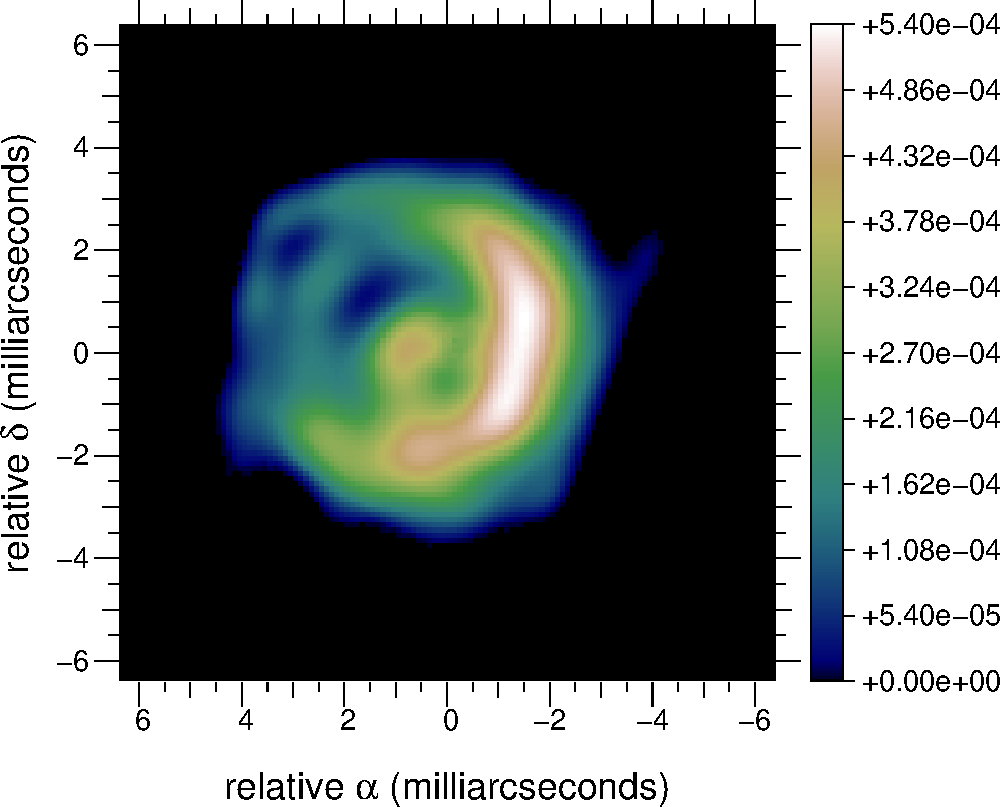
\includegraphics[height=30mm]{fig4c} &
  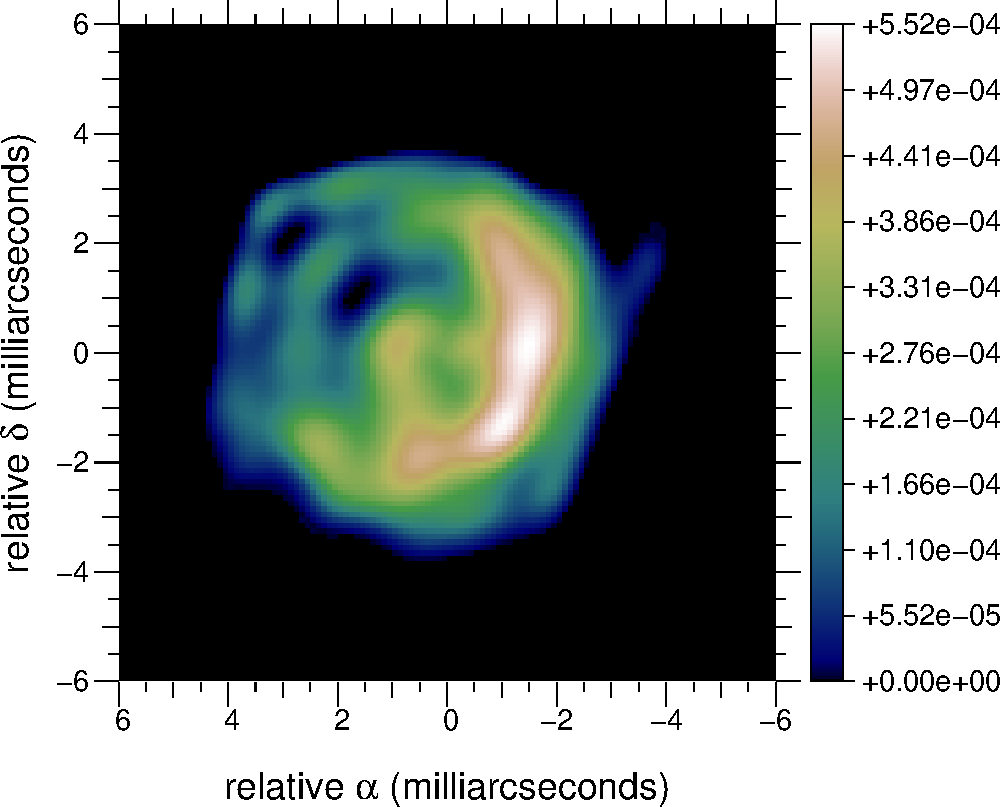
\includegraphics[height=30mm]{fig4d}\\
  \end{tabular}
  \caption{Image reconstruction under various regularization levels.
    Algorithm is \Mira with edge-preserving regularization given in
    \Eq{eq:edge-preserving-roughness} with $\epsilon=10^{-4}$ and $\mu=10^{6}$
    (top-left), $\mu=10^{5}$ (top-right), $\mu=10^{4}$ (bottom-left) and
    $\mu=3\times10^{3}$ (bottom-right).}
  \label{fig:regularization-levels}
\end{figure}

% \subsubsection{Optimization parameters}

% Starting model - often taken identical to prior model

% Disable positivity and/or normalization?

% Interactions:
% Re-center between iterations?
% Following progress
% Unsupervised reconstruction issues??


%==============================================================================
%================================================================= DISCUSSION =
%==============================================================================

\section{Discussion}

The main issues in image reconstruction from interferometric data are the
sparsity of the Fourier measurements and the lack of part of the Fourier phase
information.  The inverse problem approach appears to be suitable to describe
the most important existing algorithms in this context.  Indeed, the image
reconstruction methods can be stated as the minimization of a mixed criterion
under some strict constraints such as positivity and normalization.  Two
different types of terms appear into this criterion: likelihood terms which
enforce consistency of the model image with the data, and regularization terms
which lift the inherent degeneracies of the image reconstruction problem.
Hence the differences between the various algorithms lie in the kind of
measurements considered, in the approximations for the direct model and for
the statistics of the errors and in the prior imposed by the regularization.
For non-convex criteria which occur when the OTF is unknown or when non-linear
estimators are measured to overcome turbulence effects, the initial solution
and the optimization strategy are also key components of the algorithms.  From
a technical point of view, future developments of these algorithms will
certainly focus on global optimization and unsupervised reconstruction.
However, to fully exploit the existing instruments and those currently under
development, the most worthwhile topics to investigate are multi-spectral
imaging and making use of additional information such as a low resolution
image or partial model of the observed object.

%==============================================================================
%=============================================================== BIBLIOGRAPHY =
%==============================================================================

\newcommand{\aj}{Astron. J.} % Astronomical Journal
\newcommand{\araa}{Annual Rev. of Astron. \& Astrophys.} % Annual Review of Astron and Astrophys
\newcommand{\apj}{Astrophys. J.} % Astrophysical Journal
\newcommand{\apjl}{Astrophys. J. Lett.} % Astrophysical Journal, Letters
\newcommand{\apjs}{Astrophys. J. Suppl.} % Astrophysical Journal, Supplement
\newcommand{\ao}{Appl. Optics} % Applied Optics
\newcommand{\optlett}{Optics Lett.} % Optics Letter
\newcommand{\josa}{J.\ Opt.\ Soc.\ Am.} % Journal of the Optical Society of America
\newcommand{\josaa}{J.\ Opt.\ Soc.\ Am.\ A} % Journal of the Optical Society of America A 
\newcommand{\josab}{J.\ Opt.\ Soc.\ Am.\ B} % Journal of the Optical Society of America B 
\newcommand{\apss}{Astrophys. \& Space Science} % Astrophysics and Space Science
\newcommand{\aap}{Astron. \& Astrophys.} % Astronomy and Astrophysics
\newcommand{\aapr}{Astron. \&  Astrophys. Rev.} % Astronomy and Astrophysics Reviews
\newcommand{\aaps}{Astron. \& Astrophys. Suppl.} % Astronomy and Astrophysics, Supplement
\newcommand{\azh}{Astronomicheskii Zhurnal} % Astronomicheskii Zhurnal
\newcommand{\baas}{Bulletin of the AAS} % Bulletin of the AAS
\newcommand{\jrasc}{J. of the RAS of Canada} % Journal of the RAS of Canada
\newcommand{\memras}{Memoirs of the RAS} % Memoirs of the RAS
\newcommand{\mnras}{Monthly Notices of the RAS} % Monthly Notices of the Royal Astronomical Society
\newcommand{\pra}{Physical Rev. A: General Physics} % Physical Review A: General Physics
\newcommand{\prb}{Physical Rev. B: Solid State} % Physical Review B: Solid State
\newcommand{\prc}{Physical Rev. C} % Physical Review C
\newcommand{\prd}{Physical Rev. D} % Physical Review D
\newcommand{\pre}{Physical Rev. E} % Physical Review E
\newcommand{\prl}{Physical Rev. Lett.} % Physical Review Letters
\newcommand{\pasp}{Publications of the ASP} % Publications of the ASP
\newcommand{\pasj}{Publications of the ASJ} % Publications of the ASJ
\newcommand{\qjras}{Quarterly J. of the RAS} % Quarterly Journal of the RAS
\newcommand{\skytel}{Sky and Telescope} % Sky and Telescope
\newcommand{\solphys}{Solar Physics} % Solar Physics
\newcommand{\sovast}{Soviet Astronomy} % Soviet Astronomy
\newcommand{\ssr}{Space Science Rev.} % Space Science Reviews
\newcommand{\zap}{Zeitschrift fuer Astrophysik} % Zeitschrift fuer Astrophysik
\newcommand{\nat}{Nature} % Nature
\newcommand{\iaucirc}{IAU Cirulars} % IAU Cirulars
\newcommand{\aplett}{Astrophys. Lett.} % Astrophysics Letters
\newcommand{\apspr}{Astrophys. Space Physics Research} % Astrophysics Space Physics Research
\newcommand{\bain}{Bulletin Astronomical Institute of the Netherlands} % Bulletin Astronomical Institute of the Netherlands
\newcommand{\fcp}{Fundamental Cosmic Physics} % Fundamental Cosmic Physics
\newcommand{\gca}{Geochimica Cosmochimica Acta} % Geochimica Cosmochimica Acta
\newcommand{\grl}{Geophysics Research Lett.} % Geophysics Research Letters
\newcommand{\jcp}{J. of Chemical Physics} % Journal of Chemical Physics
\newcommand{\jgr}{J. of Geophysics Research} % Journal of Geophysics Research
\newcommand{\jqsrt}{J. of Quantitiative Spectroscopy and Radiative Transfer} % Journal of Quantitiative Spectroscopy and Radiative Transfer
\newcommand{\memsai}{Mem. Societa Astronomica Italiana} % Mem. Societa Astronomica Italiana
\newcommand{\nphysa}{Nuclear Physics A} % Nuclear Physics A
\newcommand{\physrep}{Physics Reports} % Physics Reports
\newcommand{\physscr}{Physica Scripta} % Physica Scripta
\newcommand{\planss}{Planetary Space Science} % Planetary Space Science
\newcommand{\procspie}{Proc. SPIE} % Proceedings of the SPIE

\bibliographystyle{plainnat}
\bibliography{unified_desc}

\end{document}
%------------------------------------------------------------------------------
% Local Variables:
% mode: LaTeX
% fill-column: 78
% tab-width: 8
% coding: latin-1
% End:
%------------------------------------------------------------------------------
